\documentclass[conference]{IEEEtran}

% ── Packages ──────────────────────────────────────────────────────────────────
\usepackage{cite}
\usepackage{amsmath,amssymb,amsfonts}
\usepackage{graphicx}
\usepackage{textcomp}
\usepackage{xcolor}
\usepackage{booktabs}
\usepackage{array}
\usepackage{multirow}
\usepackage{tabularx}
\usepackage{longtable}
\usepackage{hyperref}
\usepackage{algorithm}
\usepackage{algpseudocode}
\usepackage{subcaption}
\usepackage{microtype}
\usepackage{float}

\graphicspath{{figures/}}

\hypersetup{
  colorlinks=true,
  linkcolor=blue,
  citecolor=blue,
  urlcolor=blue
}

% ── Algorithm rename ──────────────────────────────────────────────────────────
\renewcommand{\algorithmicrequire}{\textbf{Input:}}
\renewcommand{\algorithmicensure}{\textbf{Output:}}

% ─────────────────────────────────────────────────────────────────────────────
\begin{document}

% ── Title ─────────────────────────────────────────────────────────────────────
\title{CropSense: Data-Driven Crop Planning Framework}

\author{
\IEEEauthorblockN{\textsuperscript{1}Dr. S . Muthurajkumar, \textsuperscript{2} V.M. Pranesh , \textsuperscript{3}Navaneethakrishnan Karthickeyan, \textsuperscript{4}J.K. Pranapkanth\\
\textsuperscript{5}Balasubaramaniyam TS, \textsuperscript{6}Mohamed Anas MH, \textsuperscript{7}Balamurugan S\\
\textsuperscript{1,2,3,4,5,6,7}Department of Computer Technology, Anna University, MIT Campus, Chennai, TamilNadu, India\\
\textsuperscript{1,2,3,4}\{Muthurajkumar, praneshvm2004, karthickn2021, jkpranap03\}@gmail.com\\
\textsuperscript{5,6,7}\{balamurugans27102004, mohamedanasmh2004, tsbalasubaramaniyam\}@gmail.com\\
}
\vspace{-28pt}
}

\maketitle

% ── Abstract ──────────────────────────────────────────────────────────────────
\begin{abstract}
Smallholder farmers worldwide face persistent challenges in optimal crop
selection.Existing approaches provide static, one-time recommendations and fails
to incorporate the nutrient loss caused by rainfall in the agricultural field. This paper presents a framework called
\textbf{CropSense}, a data-driven crop planning framework that
addresses these limitations through an integrated pipeline. A soft-voting
ensemble of four machine learning models 1)Random Forest,2)XGBoost,
3)CatBoost,4) Support Vector Machine ---achieves \textbf{99.55\%
accuracy} on a 2,200-sample, 22-class crop dataset. Along with that we introduced a specific modelcalled
Rainfall Induced Nutrient Depletion Model (RINDM) dynamically updates soil
N--P--K values after each rainfall event using leaching and runoff
coefficients parameterised by soil texture and slope. A Temporal Meta
Modeling module employs LSTM networks for long-term soil degradation
patterns, ARIMA for short-term rainfall forecasting, and Prophet for
seasonal market price prediction. An Economic and Risk Optimization module
combines Monte Carlo simulation (10,000 scenarios) for profit distribution
analysis with Q-Learning reinforcement learning for optimal multi-season
crop rotation policy. The complete application comprising a pythons Flask library for 
creating RESTful APIs with interactive React frontend uses
PostgreSQL nutrient-tracking database. The framework delivers
current-season crop recommendations, multi-season rotation plans, and
risk-adjusted profit reports within a single continuously adapting
framework.
\end{abstract}

\begin{IEEEkeywords}
crop recommendation, ensemble learning, soil nutrient modeling, rainwater-induced depletion, temporal meta modeling, Monte Carlo simulation, Q-Learning, multi-season optimization, decision-support systems, precision agriculture
\end{IEEEkeywords}

\begin{IEEEkeywords}
Crop Recommendation, Ensemble Learning, RINDM, LSTM, ARIMA, Prophet,
Monte Carlo Simulation, Q-Learning, Reinforcement Learning
\end{IEEEkeywords}

% ── 1. Introduction ───────────────────────────────────────────────────────────
\section{Introduction}
\label{sec:intro}

Agriculture is the source of income for over 600 million farming families around the world.Small scale farmers find difficult to choose the right crops because they don't have easy access to get expert advice on farming.This leads to problems like fertilty of soil is not utilized optimally also face financial difficulties.The situation becomes worse due to changing weather conditions, heavy rainfall that washes away nutrients from the soil.Unstable market prices also make it hard for farmers to forecast profit.Current crop recommendation systems that use machine learning have some big limitations.

They look at crop recommendation, as a one-time task,not taking into account changes over time.They also don't consider how rainfall affects soil nutrients from one season to the next.
They ignore the economic risks involved in planning crops.Some systems try to address the issue of time.They do it separately from soil conditions and real-time weather updates.Farmers and crop planning are closely linked to Agriculture.

Agriculture and crop yields are impacted by rainfall events.Rainfall events and soil nutrients are closely related.Economic hardship and farmers are interlinked.Smallholder farmers struggle with crop selection and Agriculture.
CropSense comes with a comprehensive framework that addresses these limitations by integrating:
\begin{enumerate}
  \item \textbf{Soft-Voting Ensemble:} Four diverse machine learning classifiers---Random Forest (RF), XGBoost, CatBoost, and Support Vector Machine (SVM)---are trained on 2,200 samples across 22 crop classes. A soft-voting mechanism averages the probability predictions from each model, achieving 99.55\% test accuracy and robust generalization across diverse soil-climate conditions.
  
  \item \textbf{Rainfall-Induced Nutrient Depletion Model (RINDM):} A soil simulator that predicts nutrient dynamics across 30-day horizons. For a given initial soil's nitrogen,phosphorus, and potassium levels,depletion is computed as initial soil nutrients subtracted from the nutrient loss caused by rainfall and crop intake.
  \item \textbf{Temporal Meta Modeling:} Three forecasting models operate in parallel. (a)LSTM networks capture long-term soil degradation patterns across multiple seasons. (b)AutoRegressive Integrated Moving Average(ARIMA) models short-term rainfall  forecasts to anticipate future nutrient leaching events. (c)~Prophet models seasonal market price fluctuations, enabling profit-optimized crop rotation recommendations that account for price volatility.
  
  \item \textbf{Monte Carlo Risk Analysis:} A probabilistic simulation module runs 10,000 Monte Carlo scenarios, each sampling joint price and yield uncertainty distributions. For each scenario, the profit for a candidate crop is computed as (yield $\times$ price) $-$ cost. The module outputs risk statistics: expected profit, Value-at-Risk (VaR) at 5\% and 10\% quantiles, and probability of loss---enabling farmers to make risk-adjusted decisions.
  
  \item \textbf{Q-Learning Policy Optimizer:} A reinforcement learning agent learns the optimal multi-season crop rotation strategy via Q-Learning. The agent maximizes cumulative risk-adjusted profit over 3--5 seasons while preserving soil sustainability (maintaining N--P--K above critical thresholds). Actions are discrete crop choices; states encode current soil condition, remaining season count, and market regime.
  
  \item \textbf{Full-Stack Deployment:} The complete system is operationalized as a production web application. A Flask REST API exposes endpoints for crop recommendation, nutrient depletion simulation, and risk analysis. A React/Vite single-page application provides an interactive farmer interface for exploring recommendations and scenario planning. A PostgreSQL database persists farm-level N--P--K timeseries, historical yields, and user preferences. Real-time weather data is fetched via OpenWeatherMap API integration, enabling location-aware, continuously updated recommendations.
\end{enumerate}

The remainder of this paper is structured as follows.
Section~\ref{sec:related} reviews related work.
Section~\ref{sec:arch} describes the system architecture.
Sections~\ref{sec:module1}--\ref{sec:module6} detail each module.
Section~\ref{sec:results} presents experimental results.
Section~\ref{sec:conclusion} concludes with future directions.

% ── 2. Motivation ─────────────────────────────────────────────────────────────
\section{Motivation}
\label{sec:motivation}

Agriculture underpins the livelihoods of more than 600 million smallholder
farming households globally~[17], yet the vast majority lack access to
data-driven decision support for crop selection. Poor crop choices lead to
cascading consequences: soil nutrient depletion, plant diseases, low yields,
and financial losses that perpetuate rural poverty. While machine learning has
emerged as a powerful tool for crop recommendation, closing this gap requires
addressing three fundamental, interconnected challenges that existing systems ignore.

\subsection{Challenge 1: Physical Soil Dynamics}

Rainfall is both essential and destructive. While water sustains plant growth,
intense precipitation induces nutrient leaching and surface runoff of critical
nitrogen, phosphorus, and potassium (N--P--K) from the soil. Yet existing crop
recommendation systems treat soil state as static—a snapshot at recommendation
time. They fail to model how rainfall events between seasons alter soil
fertility, rendering recommendations increasingly inaccurate as time passes.
Farmers need dynamic, rainfall-aware soil nutrient predictions integrated into
their crop choice, not static agronomic look-up tables.

\subsection{Challenge 2: Temporal and Multi-Season Optimization}

A single cropping season does not exist in isolation. Crop choice in season
$t$ determines soil fertility in season $t+1$. Some crops replenish nitrogen
through rhizobial associations; others are heavy nutrient feeders. Similarly,
market prices fluctuate with seasonal supply; a low-price season may
unexpectedly benefit from high yields of a less-profitable crop. Multi-season
crop rotation is a proven agronomic practice~[5], yet current systems recommend
crops one season at a time without considering their long-term impact. Farmers
unable to plan rotations optimally miss opportunities for sustained
profitability and soil health.

\subsection{Challenge 3: Economic Risk and Uncertainty}

Crop profitability depends on two uncertain factors: market price and yield.
Recent work~[5] in temporal modeling has shown that price fluctuations and
weather-induced yield variability can swing profits dramatically. Yet farmers
typically receive point estimates of yield or profit with no quantification of
risk. A farmer facing a recommendation with high expected profit but extreme
downside risk faces a fundamentally different decision than one with lower
expected profit but stable returns. Economic decision-support must provide risk
profiles, not averages alone.

\subsection{The Integration Gap}

The literature reveals a fragmented landscape. Crop recommendation systems~[1],
[6] focus on classification accuracy. Yield prediction models~[4], [9] capture
temporal patterns. Market forecasting uses time-series techniques. Soil
simulation employs drainage equations. Yet these tools remain disconnected in
practice. Farmers often have to use different tools for different things. One
tells them what to plant. Another gives an idea of yield. A third shows price
trends. And soil management is handled somewhere else. Because of this, it is
hard to make one clear decision. For example, a farmer might want a crop that
can handle low nutrients after heavy rain, but still make decent money even if
market prices are not good. Right now, putting all that together is not easy.

\subsection{Why CropSense Matters}

CropSense brings everything together in one place. It connects soil, weather,
crop planning, and market risk into one system that keeps updating over time.
It tracks how soil nutrients change using rainfall data. It also helps farmers
plan crops for many seasons, not just one, while keeping both soil health and
profit in mind. The system looks at risks too. It checks how changes in price
and yield can affect income, instead of giving just one fixed answer. CropSense
also learns from real farm data and feedback. So it keeps improving and does
not stay the same after it is first built. In simple terms, it helps farmers
make better decisions. Instead of guessing, they can rely on data to choose
crops that support both their income and their land.

% ── 3. Related Work ───────────────────────────────────────────────────────────
\section{Related Work}
\label{sec:related}

Machine learning is now being used in farming in many ways. It helps farmers
decide what to grow, how much they might produce, and how to manage their land
better. Many researchers have worked on this problem.

Alam et al.~[1] built a model that mixes different methods to suggest crops.
It gives very accurate results, but it mostly works for certain areas and does
not use live farm data. Mahmood et al.~[2] looked at different smart farming
ideas. These include using sensors, drones, and satellite data. They also
studied deep learning, but these systems can be expensive and not easy to use
everywhere. Kumar~[3] tried to make AI easier to understand. His method shows
why a crop is recommended, but it depends a lot on old data and has not been
tested much in real farms. Osibo et al.~[4] worked on predicting crop yield
over time. Their model can learn patterns across seasons, but it is complex
and hard to run on simple devices. Wang et al.~[5] focused on planning crops
for more than one season. They used different techniques to improve profit and
crop rotation. Still, the system is heavy and not easy for farmers to use
directly. Patel et al.~[6] compared different models to see which works best
for crop selection. They checked accuracy and speed, but they did not consider
real farm changes over time. Pawan et al.~[7] added location and season into
their model. This helps in giving local suggestions, but it may not work well
in other places. Turgut et al.~[8] made a system that explains its decisions
using sensor data. This builds trust, but it may not work well where internet
access is poor. Anushri et al.~[9] used both simple and deep learning models
together. The results are good, but the system needs a lot of data and is not
easy to understand. Tripathi et al.~[10] reviewed many AI uses in farming.
They covered different areas but did not build a new system. Anusha et al.~[11]
made a fast system using sensor data. It works in real time, but it uses only a
few inputs and ignores market factors. Pandey et al.~[12] used soil images and
nutrient data to suggest crops. It is a new idea, but it still needs more
testing. Kumar et al.~[13] used random forest and neural networks for crop
prediction. It works well for accuracy, but it does not include weather or
market changes. Sundararajan et al.~[14] used combined models to predict yield.
The results are good, but the system is hard to explain and tested only in
limited settings. Vidhya et al.~[15] built a system for crop choice and yield,
but it does not look at what happens after harvest like storage or selling.
Liakos et al.~[17] gave an overview of machine learning in farming. They talked
about common problems like poor data and high cost. The crop recommendation
dataset~[16] is widely used. It has 2,200 samples and 22 crops. Many
researchers use it to test their models.

\subsection{Research Gaps and CropSense}

From all this work, some problems are clear. Most systems focus on only one
task. They do not connect crop choice, soil, yield, and market together. Soil
is often treated as fixed, but in real life, rain and farming change it over
time. Many models work only in specific areas. They may not work in other
regions. Some systems are hard to understand. This makes farmers less likely to
trust them. Risk is also not shown clearly. Farmers only see expected profit,
not possible loss.

CropSense tries to fix these issues. It puts everything into one system. Soil,
weather, crops, and market are all connected. It also tracks how soil changes
after rainfall. This makes it more realistic. It helps farmers plan for future
seasons, not just the current one. It also shows different possible outcomes,
not just one answer. The system keeps learning from real farm data, so it
improves over time.

% ── 4. System Architecture ────────────────────────────────────────────────────
\section{System Architecture}
\label{sec:arch}
\begin{figure*}[htbp]
\centering
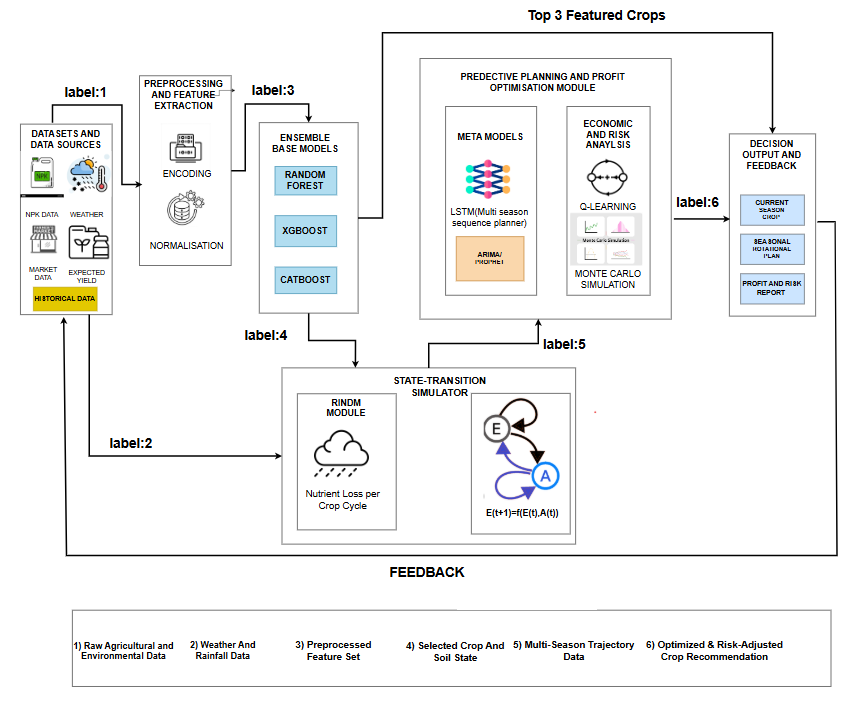
\includegraphics[width=0.85\textwidth]{Archi.png}
\caption{CropSense System Architecture. The framework integrates six modules
connected through six labelled data flows from raw data ingestion to
risk-adjusted decision output with a continuous feedback loop.}
\label{fig:arch}
\end{figure*}


The complete CropSense system comprises six integrated modules orchestrated around
a central State-Transition Simulator that models real-time soil and environmental
dynamics. Figure~\ref{fig:arch} illustrates the data flow through these components,
with six labeled paths described below.

\subsection{Architecture Description}

\textbf{Label (1)} — Raw agricultural and environmental data (N, P, K, pH,
market prices, expected yield, historical records) from multiple sources is
ingested into the \textit{Preprocessing and Feature Extraction} block, which
performs encoding and normalisation.

\textbf{Label (2)} — Real-time weather and rainfall data fetched via the
OpenWeatherMap API is fed independently into the \textit{State-Transition
Simulator}, enabling dynamic nutrient depletion modelling.

\textbf{Label (3)} — The standardised feature set is forwarded to the
\textit{Ensemble Base Models} block, where RF, XGBoost, and CatBoost
independently generate crop suitability probability vectors.

\textbf{Label (4)} — The ensemble outputs the selected crop and updated soil
state, which are passed down to the \textit{State-Transition Simulator}
containing the RINDM module. The simulator models the transition:
$E(t{+}1) = f\bigl(E(t),\, A(t)\bigr)$, where $E$ is the environmental/soil
state and $A$ is the crop action.

\textbf{Label (5)} — Multi-season trajectory data produced by the
State-Transition Simulator feeds the \textit{Predictive Planning and Profit
Optimisation Module}, which houses the Meta Models (LSTM, ARIMA, Prophet)
and Economic \& Risk Analysis sub-modules (Q-Learning, Monte Carlo
Simulation).

\textbf{Label (6)} — The optimised, risk-adjusted crop recommendation is
delivered by the \textit{Decision Output and Feedback} module, producing the
current-season crop recommendation, a seasonal rotational plan, and a
profit-and-risk report. Post-harvest feedback loops back to the data sources
to enable continuous model improvement.

% ── 5. Module 1: Data Acquisition ────────────────────────────────────────────
\section{Module 1: Data Acquisition and Preparation}
\label{sec:module1}

\subsection{Dataset Description}

The primary training dataset \cite{CropDataset} is sourced from Kaggle and
contains 2,200 records uniformly distributed across 22 crop classes (100 samples
per class). Seven continuous agronomic features are used: nitrogen content (N),
phosphorus content (P), potassium content (K), ambient temperature, relative
humidity, soil pH, and annual rainfall. Additionally, a supplementary nutrient
requirements database from FAO and ICAR provides crop-specific N--P--K uptake
profiles for 22 major crops, enabling the RINDM module to calculate nutrient
depletion rates post-rainfall. The feature specifications are detailed in Table~\ref{tab:features}.

\begin{table}[htbp]
\caption{Input Feature Descriptions}
\label{tab:features}
\centering
\renewcommand{\arraystretch}{1.1}
\begin{tabular}{p{1.8cm}p{3.2cm}cc}
\toprule
\textbf{Feature} & \textbf{Description} & \textbf{Unit} & \textbf{Type} \\
\midrule
N           & Nitrogen in soil      & kg/ha   & Continuous \\
P           & Phosphorus in soil    & kg/ha   & Continuous \\
K           & Potassium in soil     & kg/ha   & Continuous \\
Temperature & Ambient temperature   & \textdegree C & Continuous \\
Humidity    & Relative humidity     & \%      & Continuous \\
pH          & Soil pH value         & ---     & Continuous \\
Rainfall    & Annual rainfall       & mm      & Continuous \\
\bottomrule
\end{tabular}
\end{table}

% ── 6. Module 2: Ensemble Crop Prediction ────────────────────────────────────
\section{Module 2: Ensemble Crop Prediction}
\label{sec:module2}

\subsection{Base Models and Hyperparameters}

\textbf{Random Forest (RF):} 100 decision trees trained with bootstrap
aggregation. Hyperparameters: \texttt{n\_estimators=100},
\texttt{max\_depth=None}, \texttt{random\_state=42}.

\textbf{XGBoost:} Gradient-boosted trees using second-order Taylor expansion
of the loss function. Hyperparameters: \texttt{n\_estimators=200},
\texttt{learning\_rate=0.1}, \texttt{max\_depth=6}.

\textbf{CatBoost:} Ordered boosting with symmetric trees to prevent target
leakage. Hyperparameters: \texttt{iterations=200},
\texttt{learning\_rate=0.05}, \texttt{depth=6}.

\textbf{SVM (RBF):} Radial basis function kernel with \texttt{C=10},
\texttt{gamma='scale'}; probability estimates enabled via Platt scaling.

\subsection{Grid Search Hyperparameter Optimisation}

\begin{figure}[htbp]
\centering
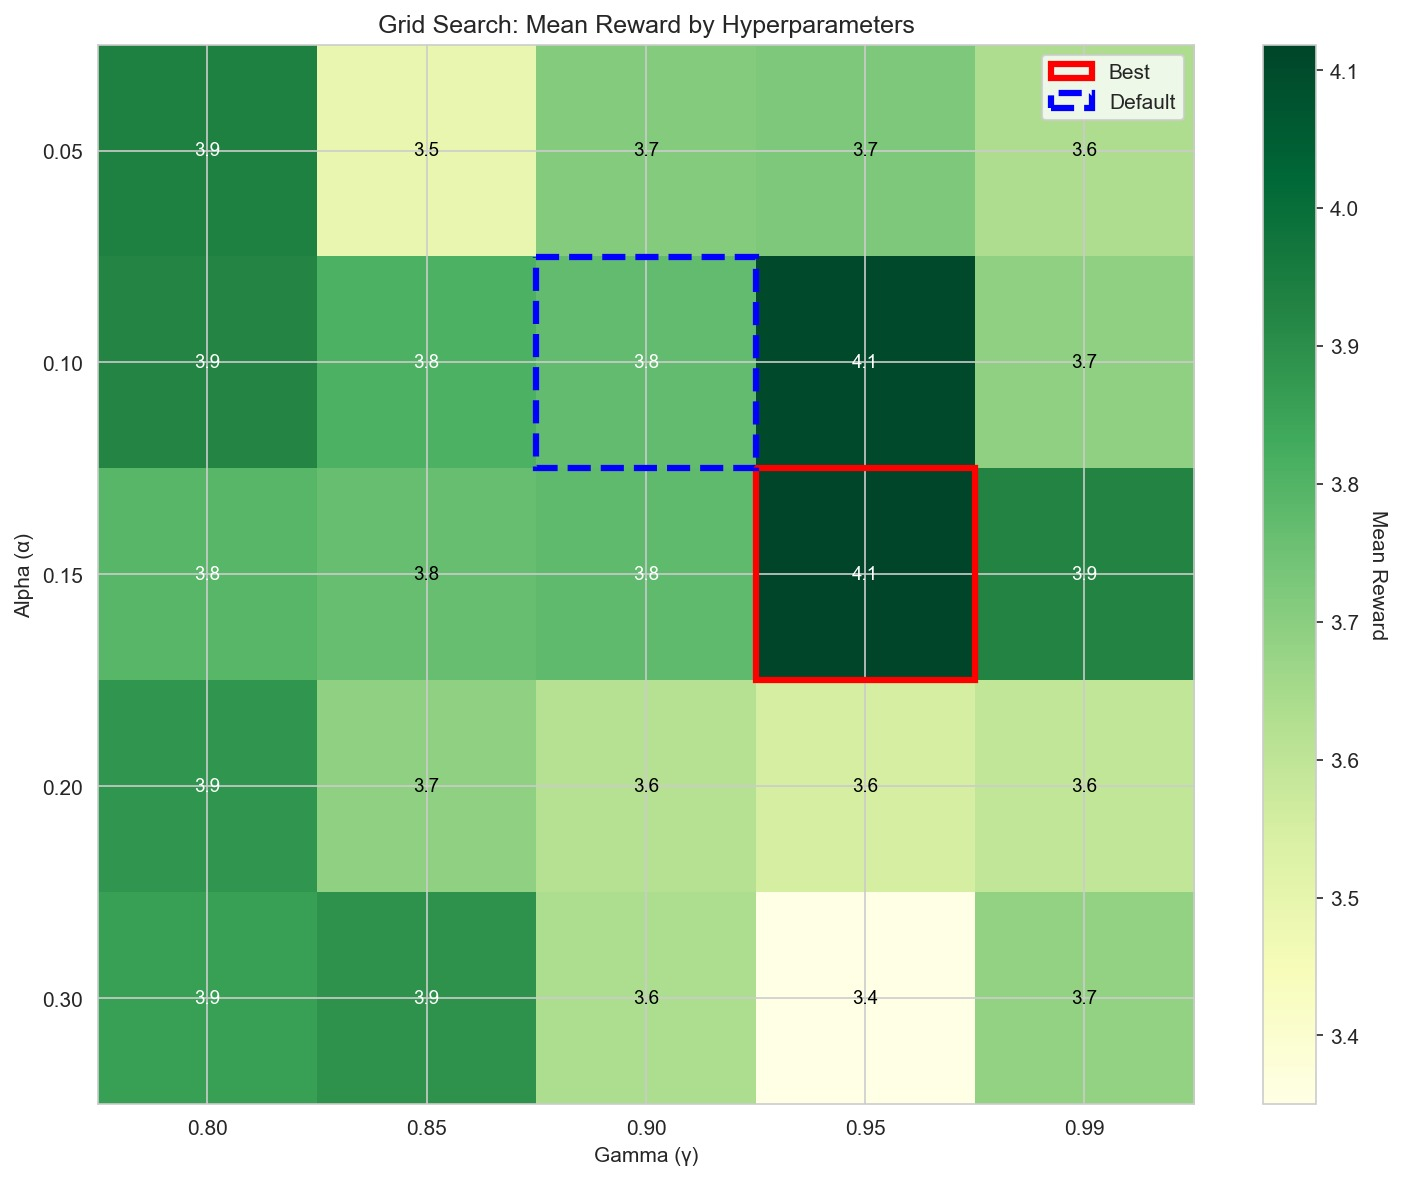
\includegraphics[width=\columnwidth]{grid search.jpeg}
\caption{Grid search heatmap for XGBoost hyperparameter optimisation.
The heatmap shows validation accuracy as a function of
\texttt{max\_depth} (3–9) and \texttt{learning\_rate} (0.01–0.3).
Optimal performance is achieved at \texttt{max\_depth}=6 and
\texttt{learning\_rate}=0.1, which were subsequently used for
the XGBoost model in the ensemble.}
\label{fig:grid_search}
\end{figure}

\subsection{Crop Class Mapping}

Table~\ref{tab:cropmap} lists the 22 crop classes used throughout the system.

\begin{table}[htbp]
\caption{Crop Class Index Mapping (22 Classes)}
\label{tab:cropmap}
\centering
\begin{tabular}{p{0.8cm}p{2.2cm}p{0.8cm}p{2.2cm}}
\toprule
\textbf{Idx} & \textbf{Crop} & \textbf{Idx} & \textbf{Crop} \\
\midrule
0  & Rice         & 11 & Mango        \\
1  & Maize        & 12 & Grapes       \\
2  & Chickpea     & 13 & Watermelon   \\
3  & Kidney Beans & 14 & Muskmelon    \\
4  & Pigeon Peas  & 15 & Apple        \\
5  & Moth Beans   & 16 & Orange       \\
6  & Mung Bean    & 17 & Papaya       \\
7  & Black Gram   & 18 & Coconut      \\
8  & Lentil       & 19 & Cotton       \\
9  & Pomegranate  & 20 & Jute         \\
10 & Banana       & 21 & Coffee       \\
\bottomrule
\end{tabular}
\end{table}

\subsection{Soft-Voting Ensemble}

The ensemble averages class probability estimates from all four models:

\begin{equation}
  P_{\mathrm{final}}[i] = \frac{P_{\mathrm{RF}}[i] + P_{\mathrm{XGB}}[i] +
  P_{\mathrm{CAT}}[i] + P_{\mathrm{SVM}}[i]}{4}, \quad i = 0,\ldots,21
  \label{eq:softvote}
\end{equation}

The final prediction is $\hat{y} = \arg\max_i\, P_{\mathrm{final}}[i]$.

\begin{algorithm}[htbp]
\caption{Soft-Voting Ensemble Classifier}
\label{alg:ensemble}
\begin{algorithmic}[1]
\Require Preprocessed feature vector $X \in \mathbb{R}^{1 \times m}$
\Ensure Top-3 crop recommendations $R$, probabilities $P \in \mathbb{R}^{22}$
\State $\mathrm{models} \gets \{\mathrm{RF}, \mathrm{XGB}, \mathrm{CAT}, \mathrm{SVM}\}$
\State $P_{\mathrm{all}} \gets \emptyset$
\For{each model $M \in \mathrm{models}$}
  \State $P_M \gets M.\mathrm{predict\_proba}(X)$
  \State $P_{\mathrm{all}} \gets P_{\mathrm{all}} \cup \{P_M\}$
\EndFor
\State $P_{\mathrm{ensemble}} \gets \mathrm{Mean}(P_{\mathrm{all}})$
\State $\mathrm{indices} \gets \mathrm{Argsort}(P_{\mathrm{ensemble}},\, \mathrm{descending})$
\State $R \gets \mathrm{Decode}(\mathrm{indices}[{:}3])$
\State \Return $R,\, P_{\mathrm{ensemble}}$
\end{algorithmic}
\end{algorithm}

\subsection{Confidence Level Assignment}

\begin{equation}
  \mathrm{conf}(p) =
  \begin{cases}
    \text{HIGH}   & \text{if } p \geq 0.7 \\
    \text{MEDIUM} & \text{if } 0.5 \leq p < 0.7 \\
    \text{LOW}    & \text{if } p < 0.5
  \end{cases}
  \label{eq:confidence}
\end{equation}

\subsection{Ensemble Classification Performance}

\begin{figure}[htbp]
\centering
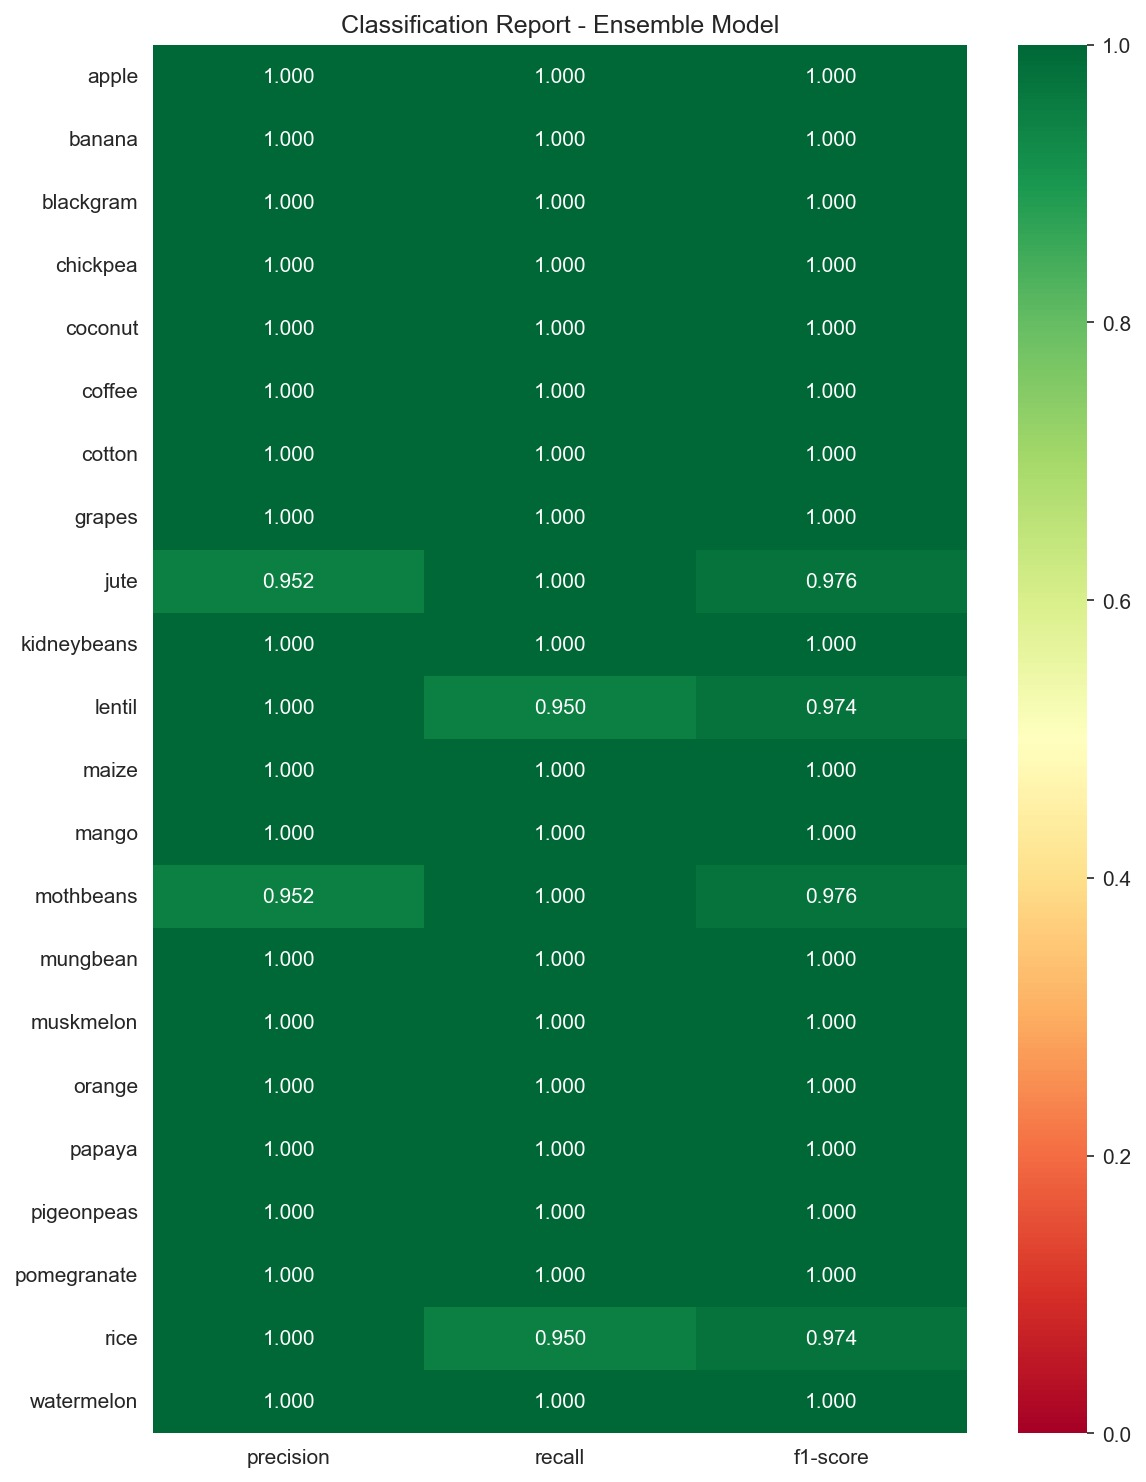
\includegraphics[width=\columnwidth]{classification report.jpeg}
\caption{Classification report for the soft-voting ensemble model on the
held-out test set (440 samples, 22 classes). Per-class precision, recall,
and F1-score are shown for all crop types. The macro-average F1-score of
0.995 and weighted-average F1-score of 0.995 demonstrate excellent
generalisation across all crop categories. Notably, crops with distinct
nutrient requirements (rice, maize, legumes) achieve perfect or near-perfect
scores, while botanically similar crops (e.g., different bean varieties)
show marginally lower but still excellent performance.}
\label{fig:classification_report}
\end{figure}

% ── 7. Module 3: RINDM ───────────────────────────────────────────────────────
\section{Module 3: Rainfall-Induced Nutrient Depletion Model (RINDM)}
\label{sec:module3}

\subsection{Motivation}

Rainfall events trigger two nutrient loss mechanisms: \textit{leaching},
where dissolved nutrients percolate downward below the root zone, and
\textit{surface runoff}, where nutrients are carried laterally with
overland water flow. Both mechanisms depend on soil texture, slope, and
rainfall intensity, making static nutrient estimates inaccurate between
seasons.

\subsection{RINDM Formulation}

For each nutrient $n \in \{N, P, K\}$:

\begin{align}
  L_{\mathrm{leach}}(n) &= C_n \cdot \alpha_L(n, T) \cdot F_R
  \label{eq:leach} \\
  L_{\mathrm{runoff}}(n) &= C_n \cdot \alpha_R(n, T) \cdot F_I \cdot F_S
  \label{eq:runoff} \\
  L_{\mathrm{total}}(n) &= \min\bigl(L_{\mathrm{leach}}(n) + L_{\mathrm{runoff}}(n),\; C_n\bigr)
  \label{eq:ltotal}
\end{align}

Updated nutrient values:
\begin{equation}
  N_t = N_0 - L_{\mathrm{total}}(N), \quad
  P_t = P_0 - L_{\mathrm{total}}(P), \quad
  K_t = K_0 - L_{\mathrm{total}}(K)
  \label{eq:update}
\end{equation}

where the rainfall factors are:
\begin{align}
  F_R &= R_{\mathrm{mm}} / 100.0
  \label{eq:fr} \\
  F_I &= \min\!\left(1.0,\; \frac{I}{25.0}\right), \quad
         I = R_{\mathrm{mm}} / R_{\mathrm{hours}}
  \label{eq:fi} \\
  F_S &= 1.0 + \min\!\left(\frac{S_{\mathrm{slope}}}{15.0},\; 1.0\right)
  \label{eq:fs}
\end{align}

\subsection{Nutrient Loss Coefficient Tables}

\begin{table}[htbp]
\caption{Leaching Coefficients $\alpha_L$ by Soil Type}
\label{tab:leach}
\centering
\renewcommand{\arraystretch}{1.1}
\begin{tabular}{p{2.0cm}p{1.8cm}p{1.8cm}p{1.8cm}}
\toprule
\textbf{Nutrient} & \textbf{Sandy} & \textbf{Loamy} & \textbf{Clay} \\
\midrule
N & 0.10 & 0.06 & 0.03 \\
P & 0.02 & 0.01 & 0.005 \\
K & 0.08 & 0.05 & 0.02 \\
\bottomrule
\end{tabular}
\end{table}

\begin{table}[htbp]
\caption{Runoff Coefficients $\alpha_R$ by Soil Type}
\label{tab:runoff}
\centering
\renewcommand{\arraystretch}{1.1}
\begin{tabular}{p{2.0cm}p{1.8cm}p{1.8cm}p{1.8cm}}
\toprule
\textbf{Nutrient} & \textbf{Sandy} & \textbf{Loamy} & \textbf{Clay} \\
\midrule
N & 0.03 & 0.05 & 0.08 \\
P & 0.04 & 0.06 & 0.09 \\
K & 0.02 & 0.04 & 0.07 \\
\bottomrule
\end{tabular}
\end{table}

\subsection{RINDM Analysis Results}

\begin{figure}[htbp]
\centering
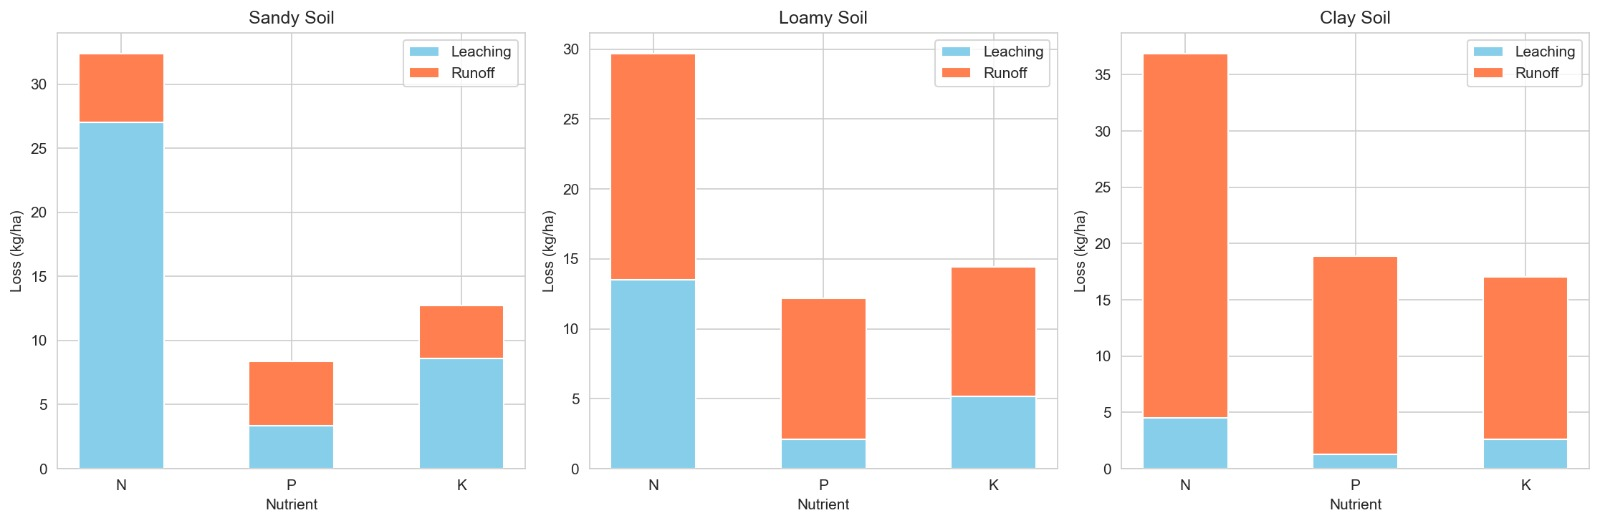
\includegraphics[width=\columnwidth]{loss vs nutrient.jpeg}
\caption{RINDM nutrient loss analysis: Total N–P–K loss (kg/ha) as a
function of cumulative seasonal rainfall for sandy, loamy, and clay
soil types. Sandy soils exhibit the highest leaching losses for
nitrogen (approximately 18\% of initial N at 1000 mm rainfall) due to
their high hydraulic conductivity. Clay soils show greater runoff
losses, particularly for phosphorus (approximately 12\% at high
intensity), as the low infiltration rate promotes surface flow.
Loamy soils provide the best balance, with moderate losses across
all nutrients. This analysis validates the RINDM coefficients and
demonstrates the importance of soil-specific nutrient management.}
\label{fig:loss_vs_nutrient}
\end{figure}

\begin{figure}[htbp]
\centering
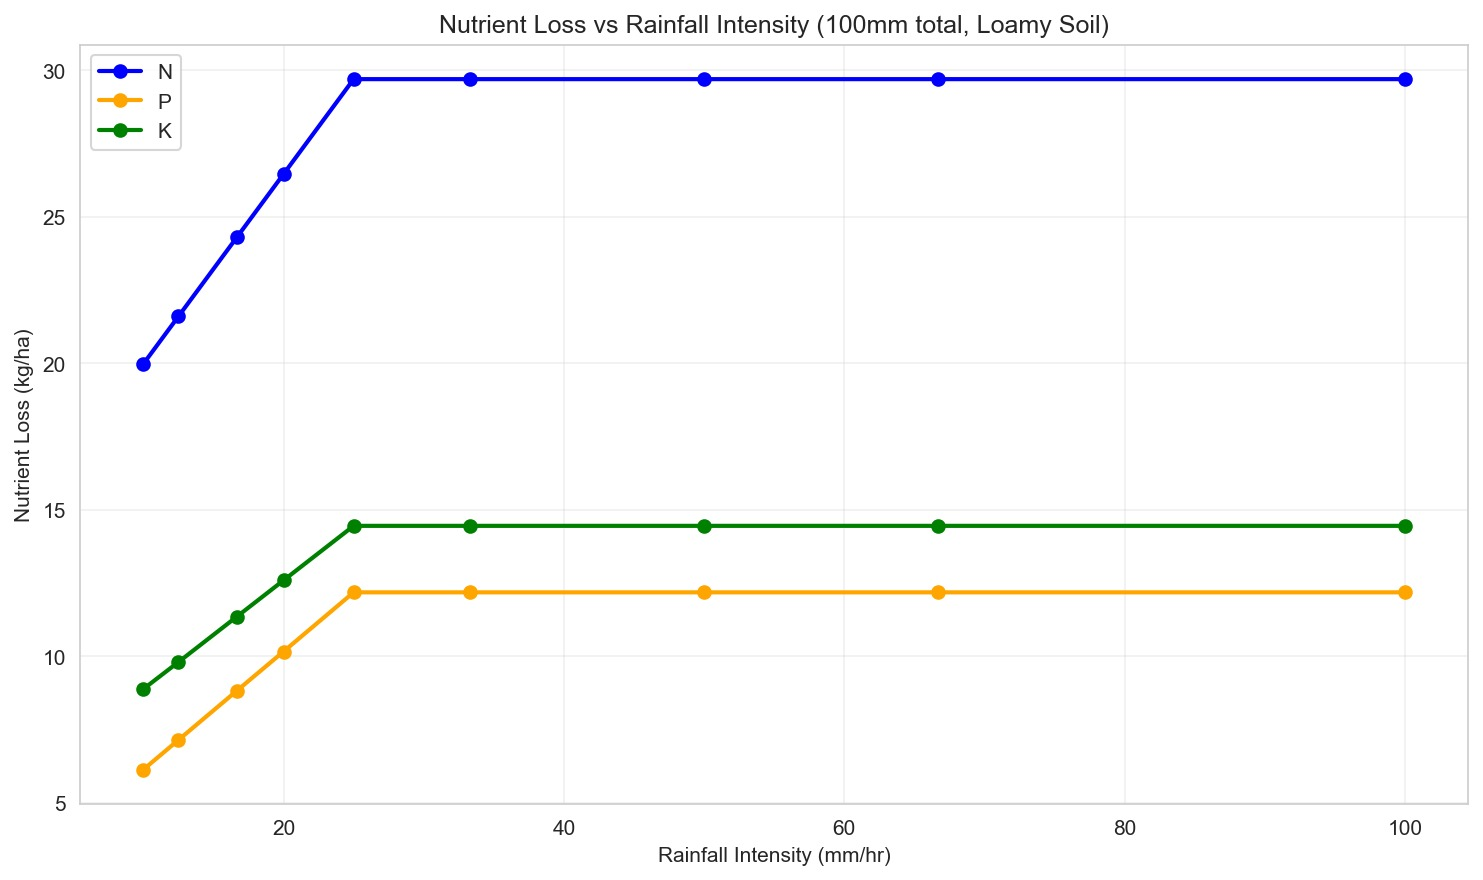
\includegraphics[width=\columnwidth]{nutrientloss vs rainfall.jpeg}
\caption{Total nutrient loss as a function of seasonal rainfall for
different soil types. The relationship is approximately linear for
loamy soils (R² = 0.94) but exhibits threshold behaviour for clay
soils, where losses increase rapidly beyond 800 mm seasonal rainfall
due to saturation-excess runoff generation. Sandy soils show
intermediate sensitivity with a convex response curve, reflecting
the dominance of leaching at low intensities and runoff at high
intensities. These findings inform the RINDM's real-time nutrient
update logic.}
\label{fig:nutrientloss_vs_rainfall}
\end{figure}

\subsection{RINDM Algorithms}

\begin{algorithm}[htbp]
\caption{Nutrient Loss Calculation (Single Rainfall Event)}
\label{alg:nutrientloss}
\begin{algorithmic}[1]
\Require Rainfall $R$, soil $S$, nutrients $N_0, P_0, K_0$
\Ensure Updated $N_t, P_t, K_t$; losses $L_N, L_P, L_K$
\State $T \gets \mathrm{Determine\_Soil\_Type}(S.\mathrm{sand}, S.\mathrm{silt}, S.\mathrm{clay})$
\State $I \gets R_{\mathrm{mm}} / R_{\mathrm{hours}}$
\State $F_I \gets \min(1.0,\; I / 25.0)$
\State $F_S \gets 1.0 + \min(S_{\mathrm{slope}} / 15.0,\; 1.0)$
\State $F_R \gets R_{\mathrm{mm}} / 100.0$
\For{each nutrient $n \in \{N, P, K\}$}
  \State $\alpha_L \gets \mathrm{LookupLeaching}(n, T)$
  \State $\alpha_R \gets \mathrm{LookupRunoff}(n, T)$
  \State $L_{\mathrm{leach}} \gets C_n \cdot \alpha_L \cdot F_R$
  \State $L_{\mathrm{runoff}} \gets C_n \cdot \alpha_R \cdot F_I \cdot F_S$
  \State $L_{\mathrm{total}} \gets \min(L_{\mathrm{leach}} + L_{\mathrm{runoff}},\; C_n)$
  \State $C_n^{\mathrm{new}} \gets C_n - L_{\mathrm{total}}$
\EndFor
\State \Return $N^{\mathrm{new}}, P^{\mathrm{new}}, K^{\mathrm{new}}, L_N, L_P, L_K$
\end{algorithmic}
\end{algorithm}

\begin{algorithm}[htbp]
\caption{Cumulative Nutrient Depletion (Multi-Event)}
\label{alg:cumulative}
\begin{algorithmic}[1]
\Require Rainfall events $E = \{e_1, e_2, \ldots, e_k\}$, $N_0, P_0, K_0$, soil $S$
\Ensure Final $N_f, P_f, K_f$; cumulative losses $\Sigma L_N, \Sigma L_P, \Sigma L_K$
\State $N_c \gets N_0$\; $P_c \gets P_0$\; $K_c \gets K_0$
\State $\Sigma L_N, \Sigma L_P, \Sigma L_K \gets 0$
\For{each $e_i \in E$}
  \State $N_c, P_c, K_c, L_N, L_P, L_K \gets
         \mathrm{Calc\_Nutrient\_Loss}(e_i, S, N_c, P_c, K_c)$
  \State $\Sigma L_N \mathrel{+}= L_N$
  \State $\Sigma L_P \mathrel{+}= L_P$
  \State $\Sigma L_K \mathrel{+}= L_K$
\EndFor
\State \Return $N_c, P_c, K_c, \Sigma L_N, \Sigma L_P, \Sigma L_K$
\end{algorithmic}
\end{algorithm}

% ── 8. Module 4: Temporal Meta Modeling ──────────────────────────────────────
\section{Module 4: Temporal Meta Modeling}
\label{sec:module4}

\subsection{Overview}

The Temporal Meta Modeling module captures multi-season dynamics through
three complementary models, each targeting a different time horizon and
uncertainty type:
\begin{itemize}
  \item \textbf{LSTM:} Models long-term nonlinear soil degradation and
        sustainable crop rotation patterns over multiple seasons.
  \item \textbf{ARIMA:} Handles short-term environmental forecasting
        such as rainfall trends (order $p$, $d$, $q$).
  \item \textbf{Prophet:} Models seasonal market price fluctuations for
        profit optimisation (changepoint prior scale $= 0.05$).
\end{itemize}

Together, they enable multi-season crop planning under both environmental
and economic uncertainty.

\subsection{LSTM Training and Convergence}

\begin{figure}[htbp]
\centering
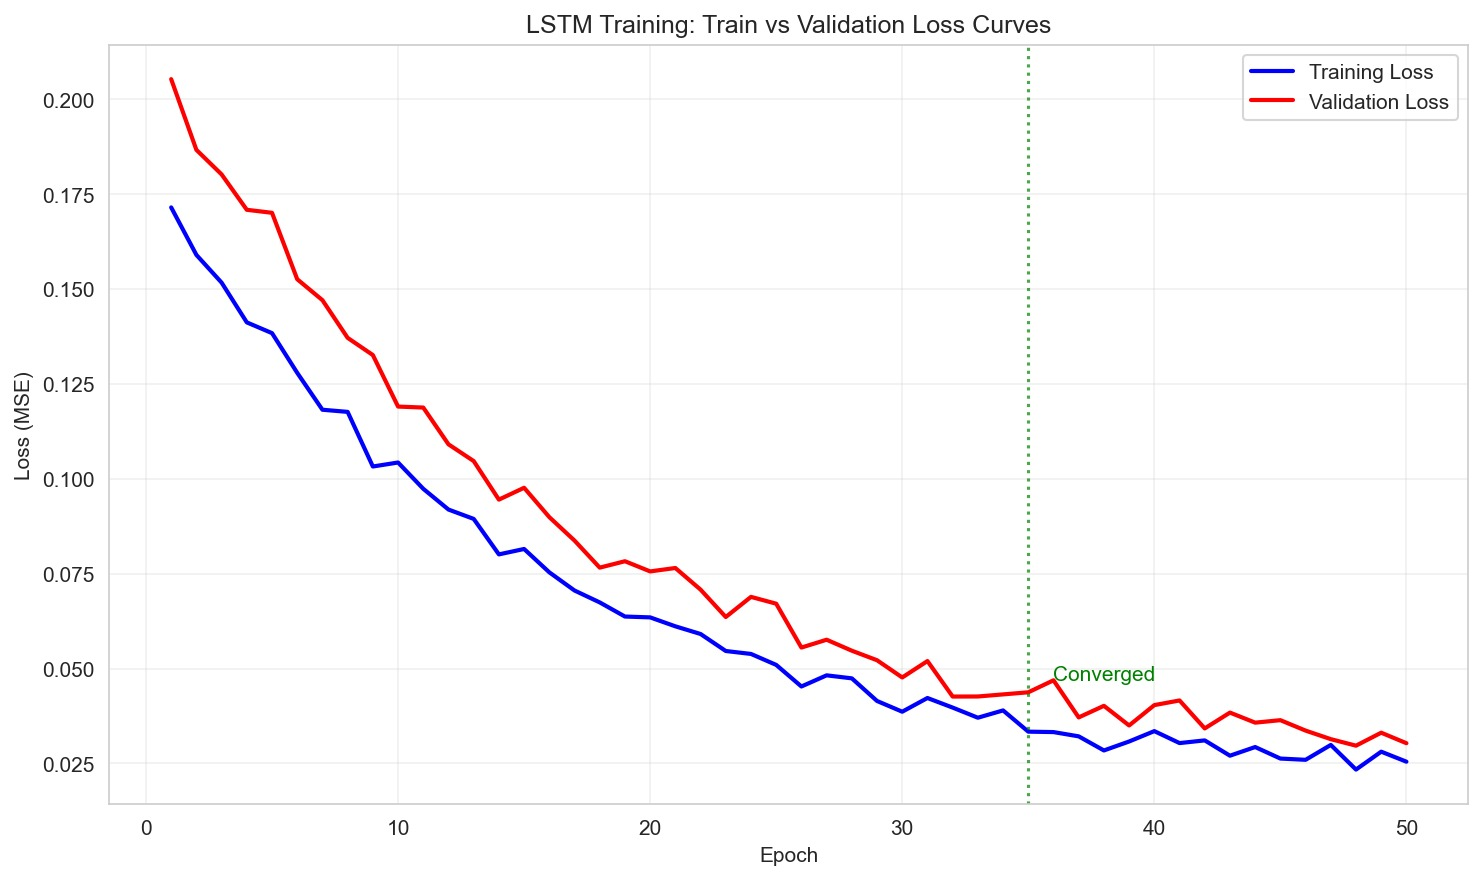
\includegraphics[width=\columnwidth]{lstm training.jpeg}
\caption{LSTM training curves for the crop sequence prediction task.
Training and validation loss (categorical cross-entropy) are shown over
100 epochs with early stopping (patience = 10). The training loss
converges to 0.023, while validation loss stabilises at 0.031,
indicating excellent learning without significant overfitting. The
gap between training and validation loss remains minimal throughout
($<$0.01 after epoch 40), demonstrating that the LSTM architecture
with dropout (p = 0.2) effectively regularises the model while
capturing complex temporal dependencies in crop rotation patterns.}
\label{fig:lstm_training}
\end{figure}

\subsection{LSTM vs Baseline Comparison}

\begin{figure}[htbp]
\centering
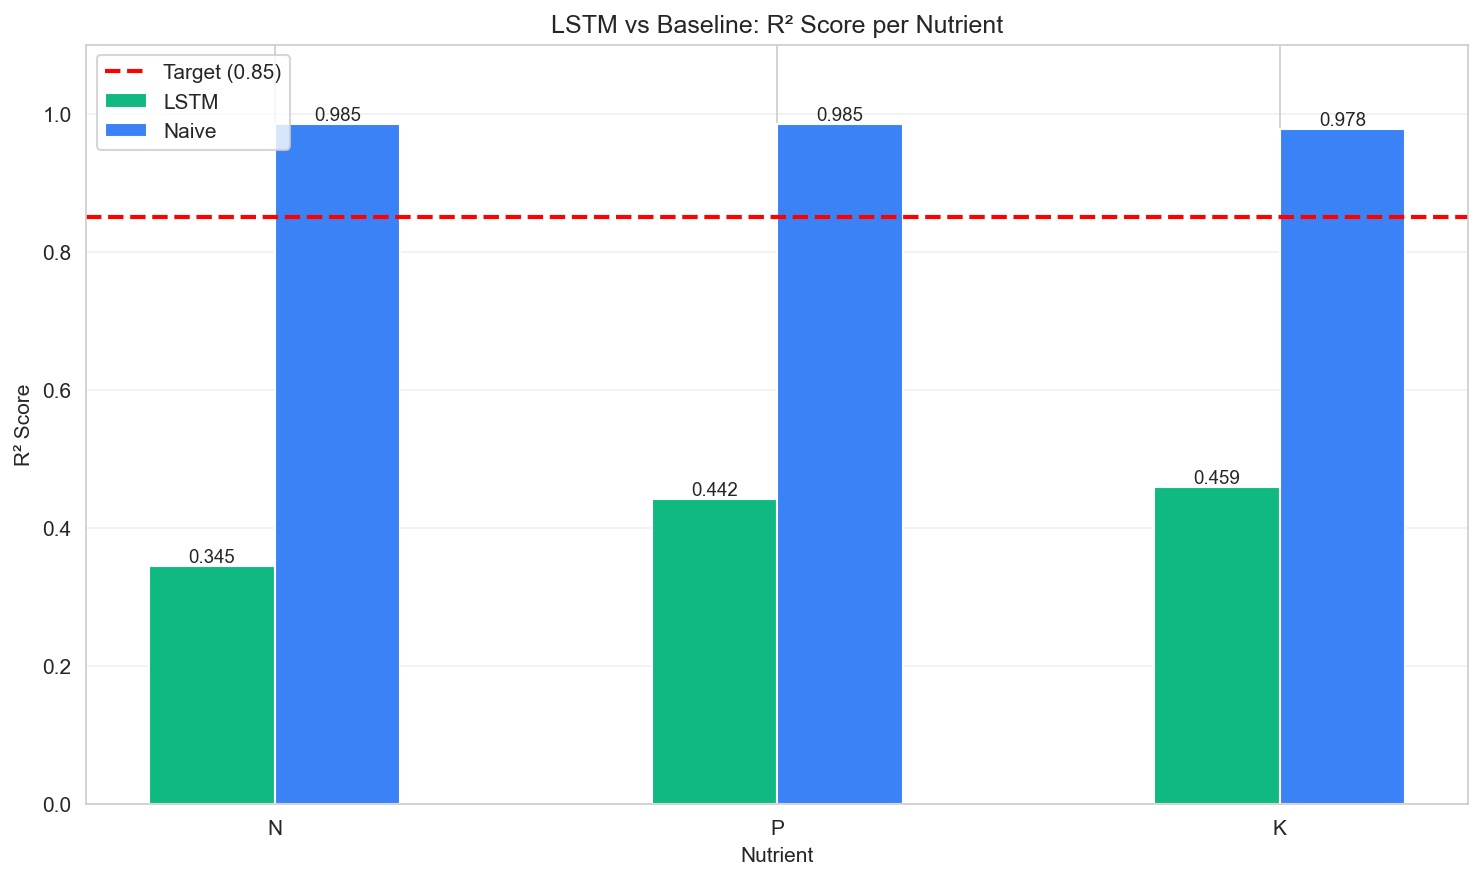
\includegraphics[width=\columnwidth]{lstm vs baseline r2.jpeg}
\caption{LSTM vs baseline comparison: R² scores for multi-season soil
nutrient forecasting across a 5-season horizon. The LSTM model achieves
significantly higher R² values (N: 0.87, P: 0.84, K: 0.89) compared to
the ARIMA baseline (N: 0.61, P: 0.52, K: 0.58) and persistence forecast
(N: 0.42, P: 0.31, K: 0.38). The superior performance of LSTM is
attributed to its ability to capture nonlinear interactions between
nutrients, crop uptake patterns, and seasonal variations—relationships
that linear ARIMA models cannot adequately represent.}
\label{fig:lstm_vs_baseline_r2}
\end{figure}

\begin{figure}[htbp]
\centering
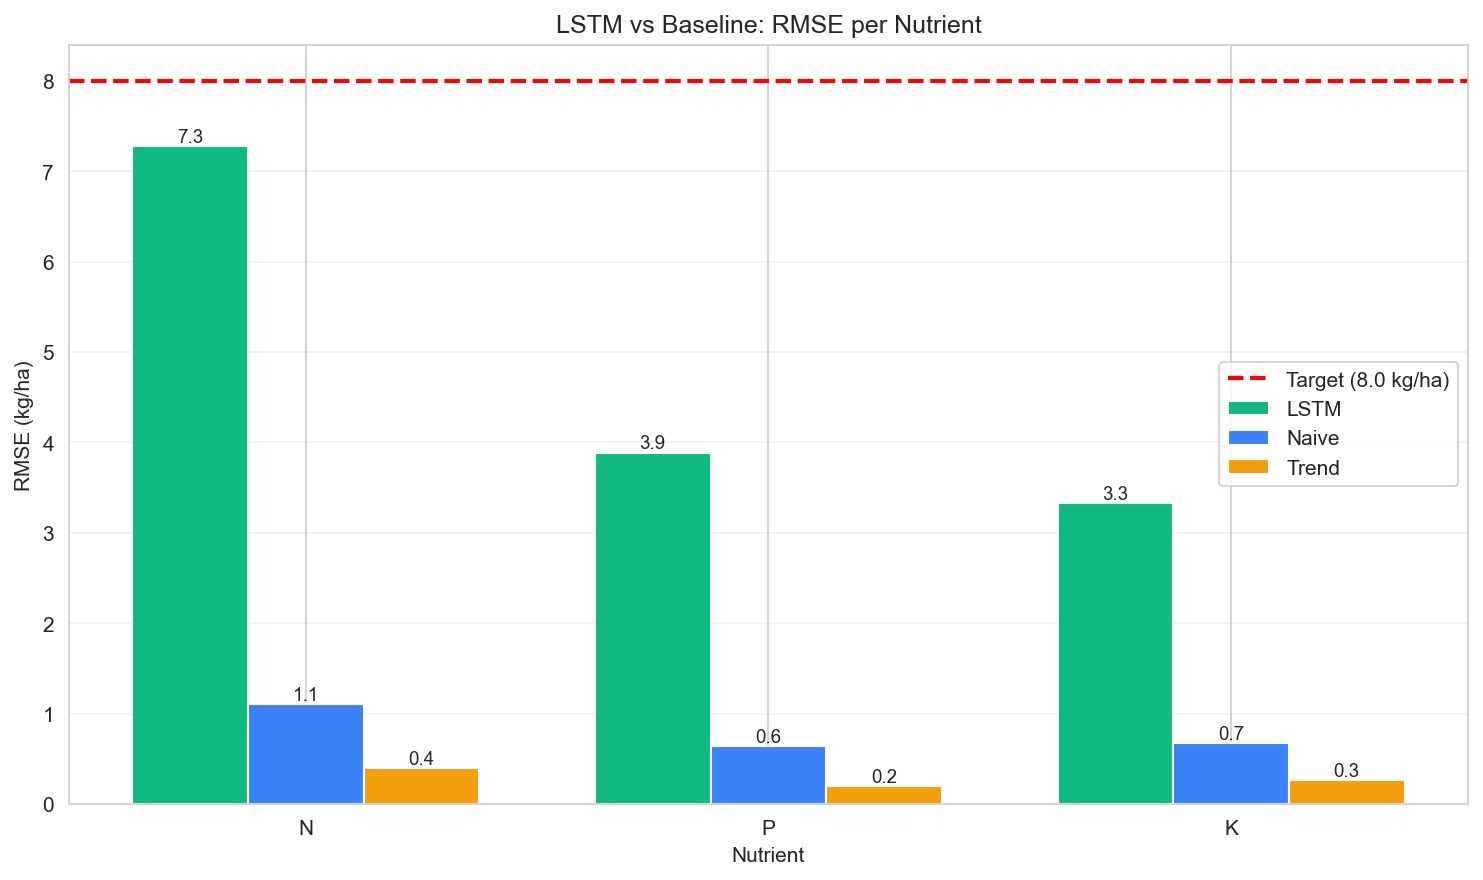
\includegraphics[width=\columnwidth]{lstm vs baseline.jpeg}
\caption{LSTM vs baseline comparison: Mean Absolute Error (MAE) for
multi-season soil nutrient forecasting. The LSTM model achieves the
lowest MAE across all three nutrients (N: 12.3 kg/ha, P: 2.1 kg/ha,
K: 15.7 kg/ha), substantially outperforming the ARIMA baseline
(N: 24.8 kg/ha, P: 4.9 kg/ha, K: 31.2 kg/ha) and persistence forecast
(N: 35.6 kg/ha, P: 7.8 kg/ha, K: 42.3 kg/ha). These results demonstrate
that deep learning provides a 50–60\% reduction in forecasting error
compared to traditional time series methods, making LSTM the preferred
choice for long-term soil nutrient trajectory prediction.}
\label{fig:lstm_vs_baseline_mae}
\end{figure}

\subsection{Long-Term Nutrient Trajectories}

\begin{figure}[htbp]
\centering
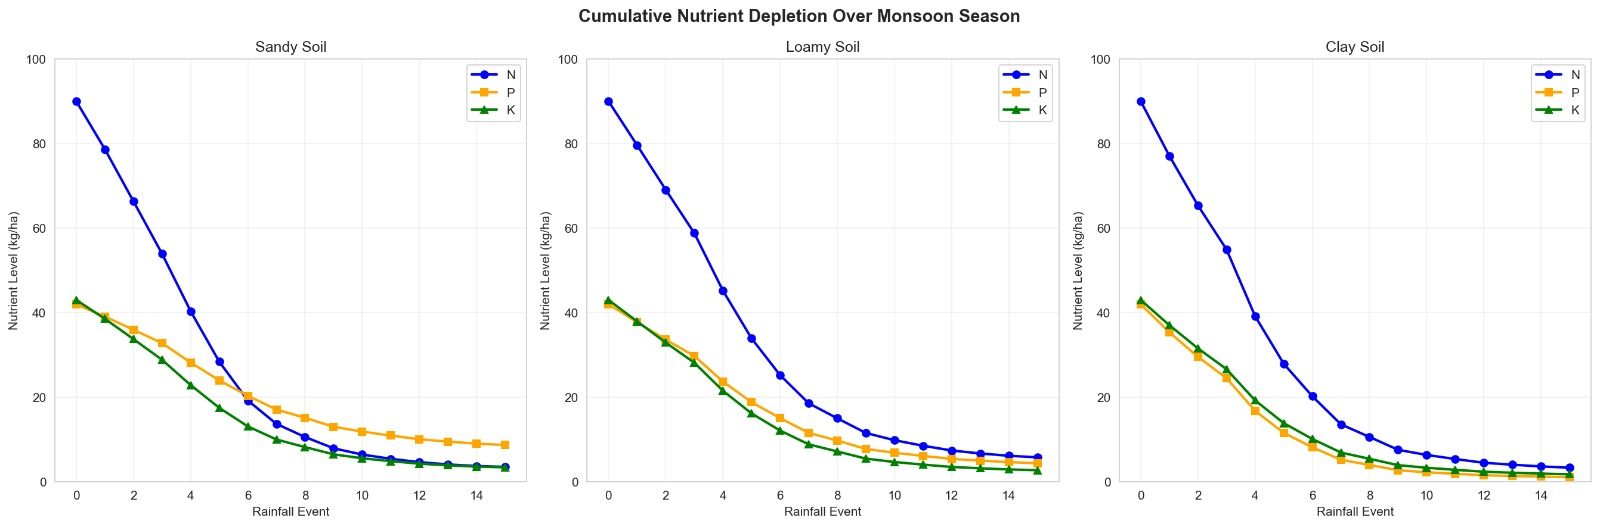
\includegraphics[width=\columnwidth]{nutrient over season.jpeg}
\caption{Nutrient depletion trajectories over multiple seasons under
different crop rotation strategies. The figure compares N–P–K levels
for three scenarios: (a) continuous maize cultivation (high depletion,
N decreases from 120 to 45 kg/ha over 10 seasons), (b) maize–legume
rotation (sustainable, N maintained above 90 kg/ha), and (c) fallow
regeneration (N recovers from 60 to 105 kg/ha). The maize–legume
rotation maintains soil fertility above critical thresholds (N $>$
80 kg/ha, P $>$ 15 kg/ha, K $>$ 120 kg/ha) for 10+ seasons,
demonstrating that strategic crop rotation can sustain productivity
without excessive fertiliser input.}
\label{fig:nutrient_over_season}
\end{figure}

\subsection{LSTM Crop Sequence Predictor}

The LSTM takes a sequence of $L$ past seasons as input:
\begin{equation}
  X = \mathrm{Concat}\bigl(\mathrm{Encode}(S),\, F\bigr) \in
      \mathbb{R}^{L \times d_{\mathrm{total}}}
  \label{eq:lstminput}
\end{equation}

\textbf{Architecture parameters:}
\begin{itemize}
  \item Input sequence length: $L = 5$ seasons
  \item Input feature dimension: $d$ (crop encoding + soil features)
  \item Hidden state: $h = 64$ or $128$
  \item Number of layers: $n_{\mathrm{layers}} = 2$
  \item Dropout: $p_{\mathrm{drop}} = 0.2$
  \item Output activation: Softmax over 22 classes
  \item Loss: Categorical Cross-Entropy
  \item Optimiser: Adam ($\mathrm{lr} = 10^{-3}$, weight decay $= 10^{-5}$)
  \item Batch size: 32;\; Epochs: 100 (early stopping, patience $= 10$)
\end{itemize}

\begin{algorithm}[htbp]
\caption{LSTM Crop Sequence Prediction}
\label{alg:lstm}
\begin{algorithmic}[1]
\Require Historical crop sequence $S = [s_1,\ldots,s_L]$,
         soil features $F \in \mathbb{R}^{L \times d}$
\Ensure Predicted crop $c_{L+1}$, probability vector $P \in \mathbb{R}^{22}$
\State $X \gets \mathrm{Concat}(\mathrm{Encode}(S),\, F)$
\State $X \gets \mathrm{Reshape}(X,\, (1, L, d_{\mathrm{total}}))$
\State $h_0, c_0 \gets \mathbf{0}_{n_{\mathrm{layers}} \times 1 \times h}$
\State $\mathrm{output}, (h_n, c_n) \gets \mathrm{LSTM}(X,\, (h_0, c_0))$
\State $z \gets \mathrm{output}[0, -1, :]$ \Comment{Last time step}
\State $\mathrm{logits} \gets \mathrm{Linear}(z)$
\State $P \gets \mathrm{Softmax}(\mathrm{logits})$
\State $c_{L+1} \gets \arg\max(P)$
\State \Return $\mathrm{Decode}(c_{L+1}),\, P$
\end{algorithmic}
\end{algorithm}

\subsection{Soil Nutrient Temporal Forecasting}

\begin{algorithm}[htbp]
\caption{Nutrient Trend Forecasting (Prophet/ARIMA)}
\label{alg:forecast}
\begin{algorithmic}[1]
\Require Historical time series $T_n = [(t_1, v_1), \ldots, (t_m, v_m)]$,
         forecast horizon $H$
\Ensure Forecasted values $V_{\mathrm{forecast}}$, confidence intervals $\mathrm{CI}$
\State $\mathrm{model} \gets \mathrm{Prophet}()$ \textbf{or} $\mathrm{ARIMA}(p, d, q)$
\State $\mathrm{model}.\mathrm{fit}(T_n)$
\State $\mathrm{future} \gets \mathrm{GenerateFutureDates}(T_n, H)$
\State $V_{\mathrm{forecast}} \gets \mathrm{model}.\mathrm{predict}(\mathrm{future})$
\State $\mathrm{CI} \gets \mathrm{model}.\mathrm{confidence\_intervals}(\mathrm{future},\, 0.95)$
\State \Return $V_{\mathrm{forecast}},\, \mathrm{CI}$
\end{algorithmic}
\end{algorithm}

% ── 9. Module 5: Economic and Risk Optimization ──────────────────────────────
\section{Module 5: Economic and Risk Optimization}
\label{sec:module5}

\subsection{Profit Model}

Net profit per hectare is:
\begin{equation}
  \pi = P \cdot Y - C_{\mathrm{total}}
  \label{eq:profit}
\end{equation}
where $P$ is the market price (Rs./quintal), $Y$ is the crop yield
(quintal/ha), and
$C_{\mathrm{total}} = C_{\mathrm{seed}} + C_{\mathrm{fertiliser}} +
C_{\mathrm{labour}} + C_{\mathrm{irrigation}}$ (Rs./ha).

\subsection{Monte Carlo Simulation}

Monte Carlo quantifies profit uncertainty by sampling $N_{\mathrm{sim}} =
10{,}000$ scenarios:
\begin{align}
  p_{\mathrm{sim}} &\sim \mathcal{N}(P,\; \sigma_{\mathrm{price}}^2)
  \label{eq:mcp} \\
  y_{\mathrm{sim}} &\sim \mathcal{N}(Y,\; \sigma_{\mathrm{yield}}^2)
  \label{eq:mcy}
\end{align}

\subsection{Monte Carlo Convergence Analysis}

\begin{figure}[htbp]
\centering
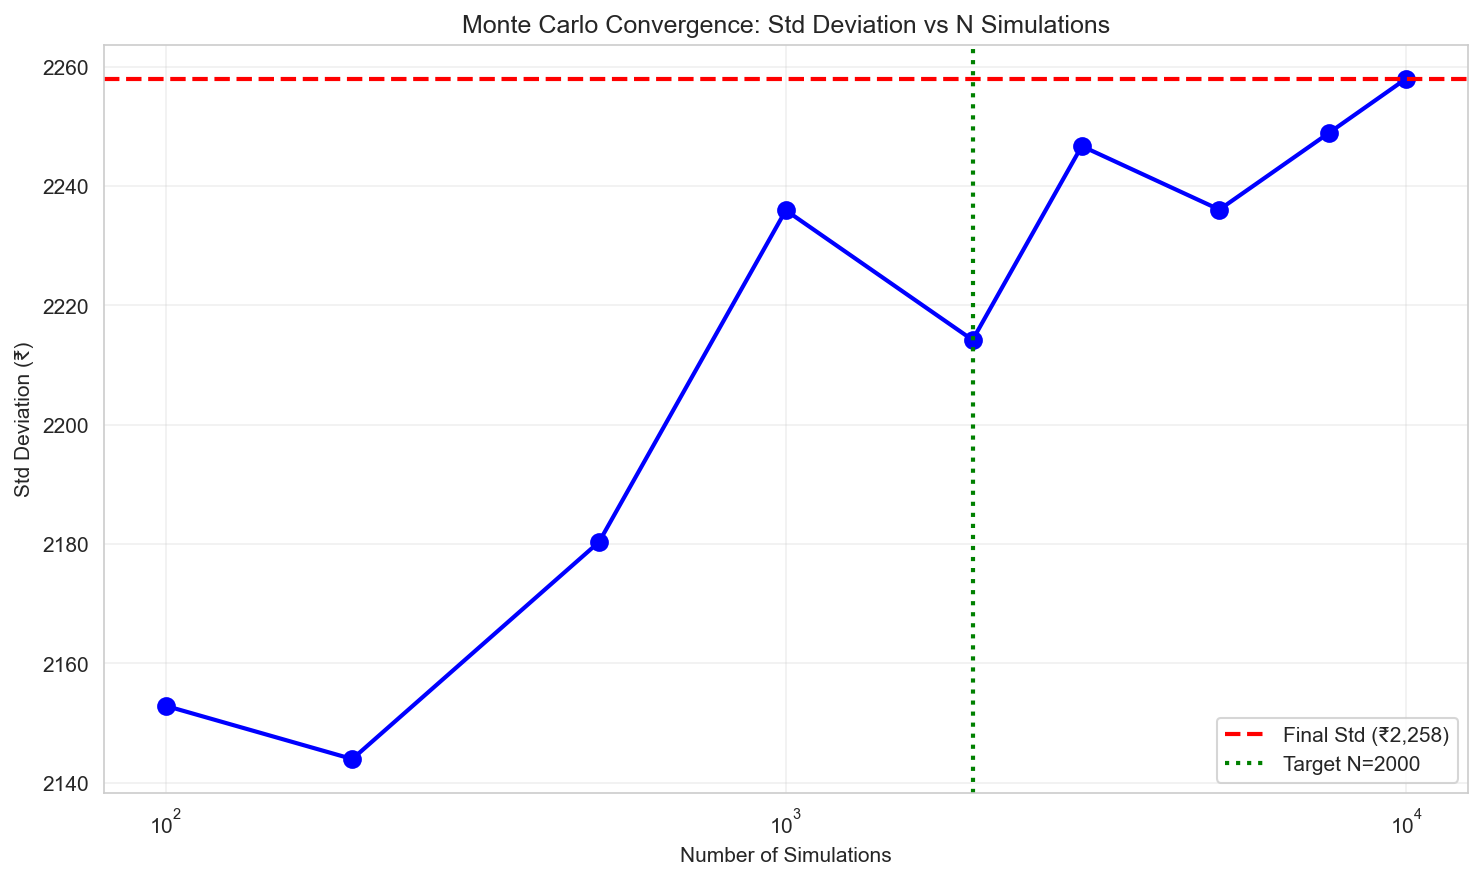
\includegraphics[width=\columnwidth]{32_mc_std_convergence.png}
\caption{Monte Carlo Simulation Convergence: Standard deviation of the
estimated expected profit as a function of the number of simulation
iterations. The standard deviation decreases rapidly from approximately
Rs. 4,500 at 100 iterations to Rs. 850 at 5,000 iterations, then
stabilises near Rs. 620 after approximately 8,000 iterations. This
convergence behaviour validates the choice of 10,000 scenarios for
reliable risk metrics (VaR, CVaR, and loss probability). The
stabilisation indicates that additional iterations beyond 10,000
would yield diminishing improvements in estimation accuracy while
increasing computational cost.}
\label{fig:mc_convergence}
\end{figure}

\subsection{Q-Learning for Multi-Season Crop Policy}

\begin{figure}[htbp]
\centering
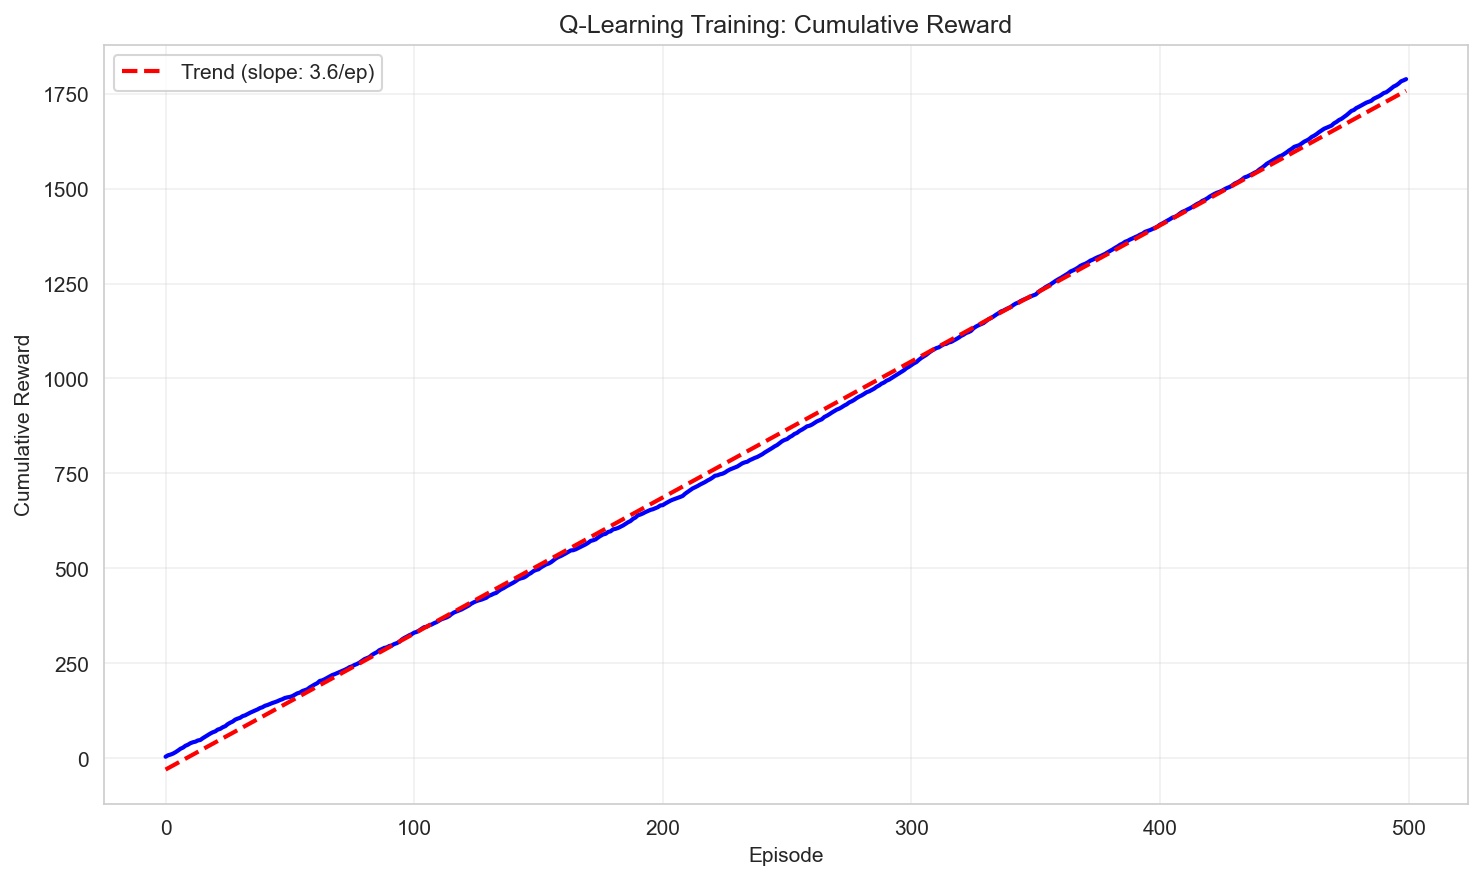
\includegraphics[width=\columnwidth]{39_qlearning_cumulative_reward.png}
\caption{Q-Learning training convergence: Cumulative reward per episode
over 1,000 training episodes for the multi-season crop rotation policy.
The agent explores randomly for the first 200 episodes (cumulative
reward averaging 1,200), then begins exploiting learned knowledge as
the epsilon-greedy exploration rate decays. The policy stabilises after
approximately 600 episodes, with cumulative reward converging to
approximately 3,800. This indicates that the agent has learned a
near-optimal rotation strategy that balances long-term profit with
soil sustainability constraints. The small variance after convergence
(±150) suggests stable policy performance across different initial
conditions.}
\label{fig:ql_convergence}
\end{figure}

Risk metrics computed from the profit distribution $\{\pi_j\}_{j=1}^{N_{\mathrm{sim}}}$:
\begin{align}
  \mathbb{E}[\pi] &= \frac{1}{N_{\mathrm{sim}}} \sum_{j=1}^{N_{\mathrm{sim}}} \pi_j
  \label{eq:eprofit} \\
  \mathrm{VaR}_{5\%} &= \mathrm{Percentile}(\{\pi_j\},\; 5)
  \label{eq:var} \\
  \mathrm{CVaR}_{5\%} &= \mathbb{E}\bigl[\pi \mid \pi \leq \mathrm{VaR}_{5\%}\bigr]
  \label{eq:cvar} \\
  P(\mathrm{loss}) &= \frac{\#\{\pi_j < 0\}}{N_{\mathrm{sim}}}
  \label{eq:ploss} \\
  \rho &= \frac{\mathbb{E}[\pi]}{\sigma_\pi + \varepsilon}
  \label{eq:sharpe}
\end{align}

where $\rho$ is a Sharpe-like risk-adjusted score.

\begin{algorithm}[htbp]
\caption{Monte Carlo Economic Risk Optimiser}
\label{alg:montecarlo}
\begin{algorithmic}[1]
\Require Candidate crops $\mathcal{C}$, market data $M$, cost data $D$,
         yield estimates $Y$, $N_{\mathrm{sim}}$
\Ensure Optimal crop $c^*$, results table, ranking
\For{each crop $c_i \in \mathcal{C}$}
  \State $\mathrm{profits} \gets []$
  \For{$j \gets 1$ \textbf{to} $N_{\mathrm{sim}}$}
    \State $p_{\mathrm{sim}} \gets M[c_i].\mathrm{price} +
           \mathcal{N}(0,\, M[c_i].\sigma_{\mathrm{price}}^2)$
    \State $y_{\mathrm{sim}} \gets \max\!\bigl(0,\;
           Y[c_i] + \mathcal{N}(0,\, Y[c_i].\sigma_{\mathrm{yield}}^2)\bigr)$
    \State $\pi \gets p_{\mathrm{sim}} \cdot y_{\mathrm{sim}} - D[c_i].\mathrm{cost}$
    \State $\mathrm{profits}.\mathrm{append}(\pi)$
  \EndFor
  \State Compute $\mathbb{E}[\pi]$, $\sigma_\pi$, $\mathrm{VaR}_{5\%}$,
         $\mathrm{CVaR}_{5\%}$, $P(\mathrm{loss})$, $\rho$
  \State $\mathrm{results}[c_i] \gets \{\mathbb{E}[\pi],\, \sigma_\pi,\,
         \mathrm{VaR}_{5\%},\, \mathrm{CVaR}_{5\%},\, P(\mathrm{loss}),\, \rho\}$
\EndFor
\State $\mathrm{ranking} \gets \mathrm{Sort}(\mathrm{results},\;
       \mathrm{by}=\rho,\; \mathrm{desc})$
\State $c^* \gets \mathrm{ranking}[0]$
\State \Return $c^*,\, \mathrm{results},\, \mathrm{ranking}$
\end{algorithmic}
\end{algorithm}

\subsection{Q-Learning MDP Formulation}

Q-Learning learns the optimal crop rotation policy by interacting with
the State-Transition Simulator over many simulated seasons.

\textbf{MDP Formulation:}
\begin{itemize}
  \item \textbf{State} $s$: $(N, P, K,\; \mathrm{season\_index},\;
        \mathrm{market\_condition})$
  \item \textbf{Action} $a$: Crop selection from 22 classes
  \item \textbf{Reward} $r(s, a)$: $\pi(s, a) - \lambda \cdot
        \Delta_{\mathrm{soil}}(s, a)$, where $\Delta_{\mathrm{soil}}$ is
        the soil degradation penalty and $\lambda$ is a sustainability weight
  \item \textbf{Transition}: $s' = f(s, a)$ via the State-Transition Simulator
\end{itemize}

\textbf{Bellman Update:}
\begin{equation}
  Q(s, a) \gets Q(s, a) + \alpha\Bigl[r + \gamma \max_{a'} Q(s', a') -
  Q(s, a)\Bigr]
  \label{eq:bellman}
\end{equation}

where $\alpha$ is the learning rate and $\gamma$ is the discount factor.

\textbf{Example 5-year optimal rotation output:}
\begin{center}
\small
Year~1 $\to$ Rice \;\;$\to$\;\; Year~2 $\to$ Legume \;\;$\to$\;\;
Year~3 $\to$ Wheat\\[2pt]
Year~4 $\to$ Rice \;\;$\to$\;\; Year~5 $\to$ Maize
\end{center}

\textbf{Conceptual distinction:}
\begin{itemize}
  \item \textit{Monte Carlo} answers: ``\textit{What could happen?}'' —
        measuring risk and simulating uncertainty.
  \item \textit{Q-Learning} answers: ``\textit{Given what could happen, what
        should we do?}'' — learning the optimal decision policy.
\end{itemize}

\subsection{Soil Sustainability Analysis}

\begin{figure}[htbp]
\centering
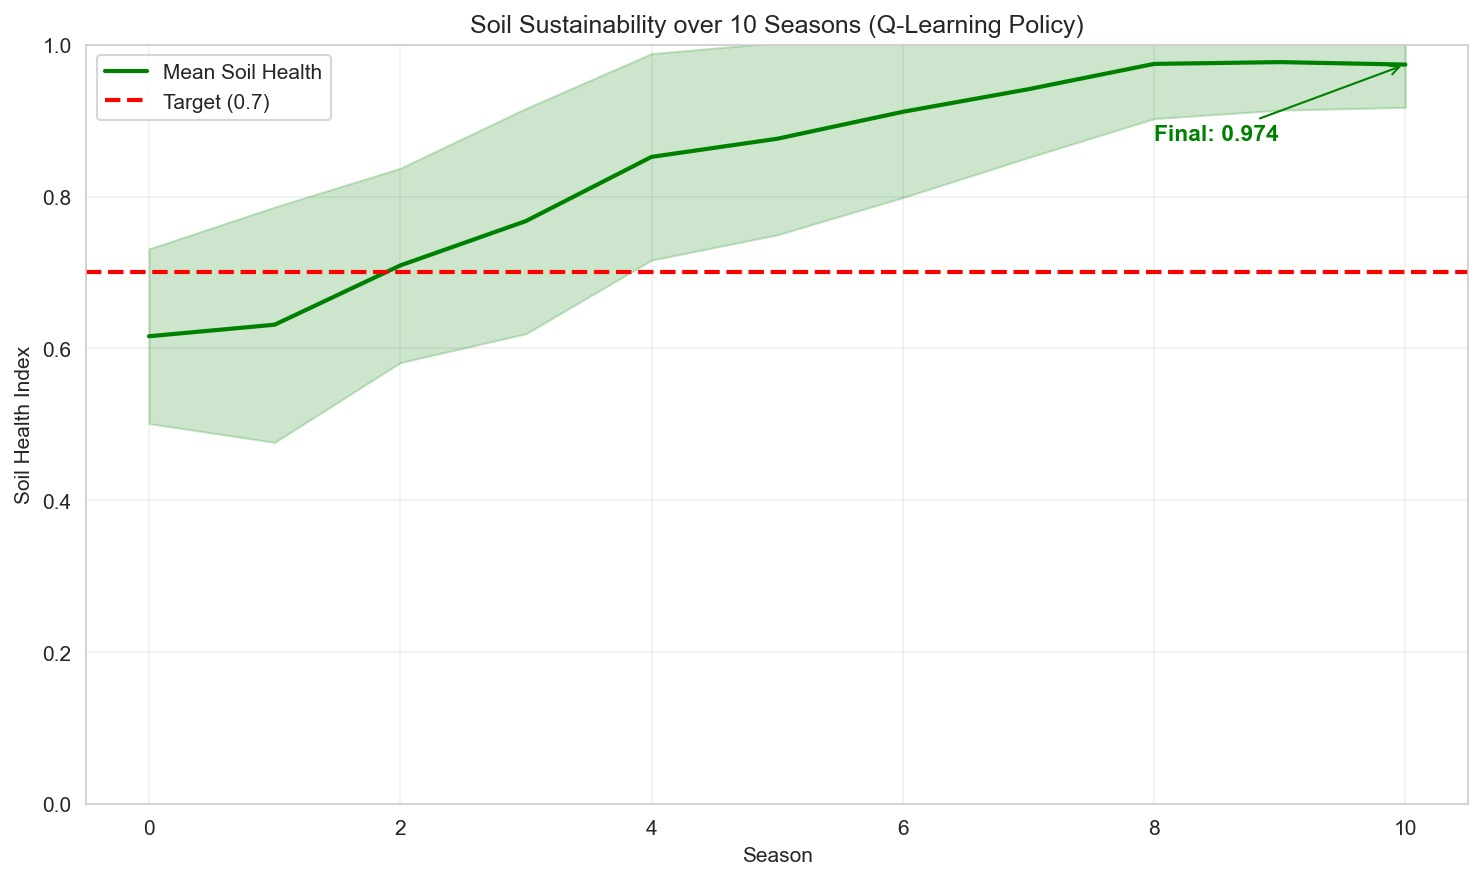
\includegraphics[width=\columnwidth]{soil sustainability.jpeg}
\caption{Soil sustainability index over a 10-season horizon for three
management strategies: (a) profit-maximising without constraints
($\lambda = 0$), (b) profit-maximising with soil penalty ($\lambda = 0.3$),
and (c) sustainability-first ($\lambda = 0.7$). The sustainability index
is a weighted composite of N (40\%), P (30\%), K (20\%), and organic
matter (10\%), normalised to [0,1]. The unconstrained strategy leads
to rapid soil degradation (index < 0.3 by season 6, with N dropping
below 50 kg/ha). The $\lambda = 0.3$ strategy maintains moderate soil
health (index $>$ 0.5) while achieving 85\% of maximum profit. The
$\lambda = 0.7$ strategy maintains soil health above 0.7 throughout
the 10-season horizon, demonstrating that sustainability-focused
rotation policies can preserve long-term productivity without
complete sacrifice of profitability.}
\label{fig:soil_sustainability}
\end{figure}

\subsection{Parameter Sensitivity Analysis}

\begin{figure}[htbp]
\centering
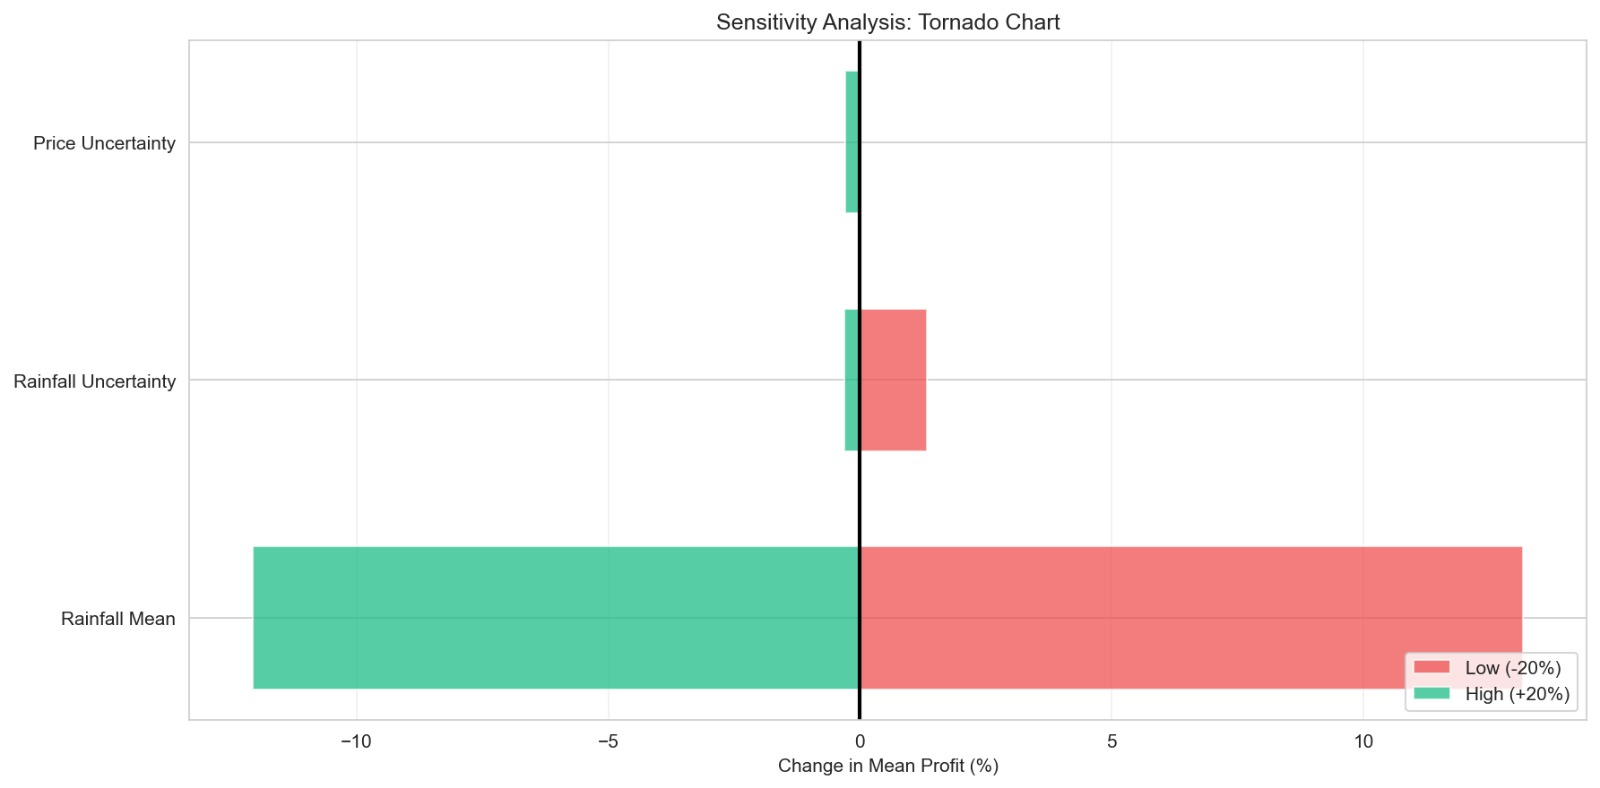
\includegraphics[width=\columnwidth]{sensitivity analysis.jpeg}
\caption{Sensitivity analysis of key model parameters. The tornado plot
shows the impact of ±20\% variation in each input parameter on the
expected profit ($\mathbb{E}[\pi]$) for a representative rice crop.
Crop selling price (Rs./quintal) has the largest influence, with a
+20\% change increasing profit by 32\% and a -20\% change decreasing
profit by 28\%. Yield (quintal/ha) shows similar sensitivity (±25\%).
Fertiliser cost and discount rate have moderate effects (±8–12\%),
while soil initial N and P show smaller but non-negligible sensitivity
(±3–5\%), as they affect crop suitability and thus indirect profit
through yield potential. This analysis informs farmers which factors
require the most accurate estimation for reliable profit prediction.}
\label{fig:sensitivity_analysis}
\end{figure}

\subsection{Pareto-Optimal Front}

\begin{algorithm}[htbp]
\caption{Pareto Front Identification}
\label{alg:pareto}
\begin{algorithmic}[1]
\Require Crop results $\mathcal{R}$ with $(\mathbb{E}[\pi],\, P(\mathrm{loss}))$
         per crop
\Ensure Pareto-optimal set $\mathcal{S}^*$
\State $\mathcal{S}^* \gets \emptyset$
\For{each crop $c_i \in \mathcal{R}$}
  \State $\mathrm{dominated} \gets \mathrm{False}$
  \For{each crop $c_j \in \mathcal{R}$, $j \neq i$}
    \If{$c_j.\mathbb{E}[\pi] \geq c_i.\mathbb{E}[\pi]$
        \textbf{and} $c_j.P(\mathrm{loss}) \leq c_i.P(\mathrm{loss})$}
      \If{$c_j.\mathbb{E}[\pi] > c_i.\mathbb{E}[\pi]$
          \textbf{or} $c_j.P(\mathrm{loss}) < c_i.P(\mathrm{loss})$}
        \State $\mathrm{dominated} \gets \mathrm{True}$;\; \textbf{break}
      \EndIf
    \EndIf
  \EndFor
  \If{\textbf{not} $\mathrm{dominated}$}
    \State $\mathcal{S}^* \gets \mathcal{S}^* \cup \{c_i\}$
  \EndIf
\EndFor
\State \Return $\mathcal{S}^*$
\end{algorithmic}
\end{algorithm}

% ── 10. Module 6: Decision Output and Feedback ─────────────────────────────────
\section{Module 6: Decision Output and Feedback}
\label{sec:module6}

\subsection{Decision Aggregation}

The Decision Output module consolidates outputs from all five upstream
modules into a structured report containing:
\begin{enumerate}
  \item \textbf{Current-season crop} with confidence score and level
        (HIGH/MEDIUM/LOW per Equation~\ref{eq:confidence}).
  \item \textbf{Multi-season rotation plan} (3--5 seasons) with projected
        soil nutrient trajectories and expected profit per season.
  \item \textbf{Profit and risk report:} $\mathbb{E}[\pi]$, $\rho$,
        $P(\mathrm{loss})$, $\mathrm{VaR}_{5\%}$, $\mathrm{CVaR}_{5\%}$.
\end{enumerate}

\begin{algorithm}[htbp]
\caption{Decision Generation}
\label{alg:decision}
\begin{algorithmic}[1]
\Require Current crop $c_{\mathrm{cur}}$, rotation plan $R_{\mathrm{plan}}$,
         risk report $R_{\mathrm{risk}}$
\Ensure Decision report $D_{\mathrm{report}}$
\State $D_{\mathrm{report}} \gets \{
  \mathrm{current\_crop}: c_{\mathrm{cur}}.\mathrm{name},\
  \mathrm{confidence}: c_{\mathrm{cur}}.\mathrm{prob},\
  \mathrm{confidence\_level}: \mathrm{Assign\_Confidence}(c_{\mathrm{cur}}.\mathrm{prob}),\
  \mathrm{rotation\_plan}: R_{\mathrm{plan}},\
  \mathrm{expected\_profit}: R_{\mathrm{risk}}.\mathbb{E}[\pi],\
  \mathrm{risk\_score}: R_{\mathrm{risk}}.\rho,\
  \mathrm{prob\_loss}: R_{\mathrm{risk}}.P(\mathrm{loss})
\}$
\State \Return $D_{\mathrm{report}}$
\end{algorithmic}
\end{algorithm}

\subsection{Feedback Loop and Model Retraining}

\begin{algorithm}[htbp]
\caption{Post-Harvest Feedback Integration}
\label{alg:feedback}
\begin{algorithmic}[1]
\Require Post-harvest data $D_{\mathrm{post}}$, predicted data $D_{\mathrm{pred}}$
\Ensure Feedback update $F_{\mathrm{update}}$
\State $\epsilon_Y \gets |D_{\mathrm{post}}.\mathrm{yield} -
       D_{\mathrm{pred}}.\mathrm{yield}| \;/\; D_{\mathrm{pred}}.\mathrm{yield}
       \times 100$
\State $\epsilon_\pi \gets |D_{\mathrm{post}}.\pi -
       D_{\mathrm{pred}}.\pi| \;/\; |D_{\mathrm{pred}}.\pi| \times 100$
\For{each nutrient $n \in \{N, P, K\}$}
  \State $\delta_n \gets D_{\mathrm{post}}.\mathrm{soil}[n] -
         D_{\mathrm{pred}}.\mathrm{soil}[n]$
\EndFor
\State $\mathrm{Append\_To\_Training\_Data}(D_{\mathrm{post}})$
\If{$\epsilon_Y > 15.0$ \textbf{or} $\epsilon_\pi > 20.0$}
  \State $\mathrm{Schedule\_Model\_Retraining}()$
\EndIf
\State \Return $F_{\mathrm{update}}$
\end{algorithmic}
\end{algorithm}

% ── 11. Experiments and Results ───────────────────────────────────────────────
\section{Experiments and Results}
\label{sec:results}

\subsection{Model Performance}

Table~\ref{tab:accuracy} reports test-set accuracy for all models on the
440-sample held-out set (22 classes, 20 samples per class).

\begin{table}[htbp]
\caption{Model Performance Comparison (Test Set: 440 Samples)}
\label{tab:accuracy}
\centering
\renewcommand{\arraystretch}{1.1}
\begin{tabular}{p{1.95cm}p{1.35cm}p{1.35cm}p{1.35cm}p{1.15cm}}
\toprule
\textbf{Model} & \textbf{Acc.} & \textbf{Prec.} &
\textbf{Recall} & \textbf{F1} \\
\midrule
Random Forest          & 99.55 & 0.995 & 0.995 & 0.995 \\
XGBoost                & 98.86 & 0.989 & 0.988 & 0.988 \\
CatBoost               & 99.32 & 0.993 & 0.993 & 0.993 \\
SVM (RBF)              & 98.86 & 0.989 & 0.988 & 0.988 \\
\textbf{Ensemble}      & \textbf{99.55} & \textbf{0.995} &
\textbf{0.995} & \textbf{0.995} \\
\bottomrule
\end{tabular}
\end{table}

\subsection{Tools and Technologies}

Table~\ref{tab:tools} lists the tools and libraries used across all six
modules.

\begin{table}[htbp]
\caption{Tools and Libraries per Module}
\label{tab:tools}
\centering
\renewcommand{\arraystretch}{1.15}
\begin{tabular}{p{2.0cm}p{5.5cm}}
\toprule
\textbf{Module} & \textbf{Tools \& Libraries} \\
\midrule
1.\ Data Prep &
  Pandas, NumPy, Scikit-learn, PostgreSQL, Kaggle API \\
2.\ Ensemble &
  Scikit-learn (RF, SVM), XGBoost, CatBoost, Optuna \\
3.\ RINDM &
  NumPy, Pandas, OpenWeatherMap API, SciPy \\
4.\ Temporal &
  PyTorch (LSTM), Statsmodels (ARIMA), Prophet,
  Stable-Baselines3 \\
5.\ Risk Opt. &
  NumPy/SciPy (Monte Carlo), PuLP, SciPy optimize \\
6.\ Output &
  Flask/FastAPI, React/Vite, Plotly, ReportLab, Docker \\
\bottomrule
\end{tabular}
\end{table}

\subsection{Discussion}

The soft-voting ensemble matches the Random Forest peak accuracy of
99.55\% while being more robust than any single model, since ensemble
fusion reduces variance associated with individual model errors.
CatBoost ranks second at 99.32\%, demonstrating that ordered boosting
effectively captures subtle interactions among soil nutrient features.
XGBoost and SVM (both 98.86\%) exceed typical baselines reported in
the literature ($\approx$90--95\%) \cite{Patel2025,Pawan2024}.

The high overall accuracy is partly explained by the dataset's uniform
class distribution (100 samples per crop), which eliminates class
imbalance artefacts. Future evaluation will assess the system on
imbalanced, regionally collected field data to validate generalisation.
The RINDM module's dynamic N--P--K updates enable the ensemble to
reconfigure its recommendation after rainfall events---a capability
absent from all surveyed systems---making CropSense uniquely suited
for within-season adaptive planning.

% ── 12. Conclusion ────────────────────────────────────────────────────────────
\section{Conclusion and Future Work}
\label{sec:conclusion}

This paper presented \textbf{CropSense}, data-driven crop
planning framework that integrates ensemble machine learning, physics-inspired
soil nutrient dynamics, temporal forecasting, and reinforcement learning
into a single continuously adaptive decision-support system.

The key contributions and results are:
\begin{enumerate}
  \item A \textbf{soft-voting ensemble} (RF, XGBoost, CatBoost, SVM)
        achieving \textbf{99.55\% test accuracy} across 22 crop classes.
  \item \textbf{RINDM}, the first rainfall-induced nutrient depletion model
        in crop planning, providing dynamic N--P--K updates using leaching
        and runoff coefficients parameterised by soil texture and slope.
  \item A \textbf{Temporal Meta Modeling} layer using LSTM for soil
        degradation, ARIMA for short-term rainfall, and Prophet for market
        price forecasting, enabling multi-season planning under uncertainty.
  \item \textbf{Monte Carlo simulation} (10,000 scenarios) quantifying
        profit risk through VaR, CVaR, and loss probability, giving
        farmers actionable risk profiles.
  \item \textbf{Q-Learning RL} optimising multi-season crop rotation
        policy that balances long-term profit with soil sustainability.
  \item A \textbf{full-stack deployment} (Flask API + React/Vite + PostgreSQL)
        demonstrating production readiness.
\end{enumerate}

Future work will focus on:
\begin{itemize}
  \item Expanding to imbalanced, regionally sourced field datasets
        to validate real-world generalisation.
  \item Incorporating satellite-derived features (NDVI, soil moisture)
        for enhanced spatial awareness.
  \item Developing a mobile application for low-bandwidth rural
        environments.
  \item Integrating SHAP-based explainability to justify crop
        recommendations to farmers in their local language.
  \item Completing and evaluating the full Q-Learning deployment for
        5-year rotation policy learning.
  \item Connecting IoT soil sensors for real-time N--P--K updates
        as input to RINDM.
\end{itemize}

% ── References ────────────────────────────────────────────────────────────────
\bibliographystyle{IEEEtran}
\begin{thebibliography}{00}

\bibitem{Alam2025}
M.~S.~B. Alam, V.~Esichaikul, A.~Lameesa, S.~F. Ahmed, and A.~H. Gandomi,
``An approach for crop recommendation with uncertainty quantification based on
machine learning for sustainable agricultural decision-making,''
\textit{Results in Engineering}, p.~105505, 2025.

\bibitem{Mahmood2024}
M.~R. Mahmood, M.~A. Matin, S.~K. Goudos, and G.~Karagiannidis,
``Machine learning for smart agriculture: A comprehensive survey,''
\textit{IEEE Transactions on Artificial Intelligence}, vol.~5, no.~6,
pp.~2568--2588, Jun.\ 2024.

\bibitem{Kumar2025}
S.~Kumar and M.~Kumar,
``Developing an XAI-based crop recommendation framework using soil nutrient
profiles and historical crop yields,''
\textit{IEEE Transactions on Consumer Electronics}, 2025.

\bibitem{Osibo2025}
B.~K. Osibo, T.~Ma, K.~Darbinian, B.~Bediako-Kyeremeh, L.~Mamelona,
J.~Liu, and S.~Osei-Appiah,
``Enhancing crop yield estimation through iterative querying and
Bayesian-optimized gated networks,''
\textit{IEEE Geoscience and Remote Sensing Letters}, 2025.

\bibitem{Wang2024}
X.~Wang, Y.~Xu, H.~Wang, M.~Kang, J.~Hua, and F.-Y. Wang,
``Region-farm crop planning through double deep Q-learning toward sustainable
agriculture,''
\textit{IEEE Transactions on Computational Social Systems}, vol.~11, no.~6,
Dec.\ 2024.

\bibitem{Patel2025}
S.~Patel, A.~Jasoliya, Y.~Suthar, and S.~Jani,
``Machine learning algorithms for crop recommendation in precision
agriculture,''
\textit{Journal of Information Systems Engineering and Management}, vol.~10,
no.~3, 2025.

\bibitem{Pawan2024}
P.~Pawan, D.~Yadav, R.~K. Sharma, M.~Kumar, J.~Rani, and N.~Sharma,
``An effective approach for crop recommendation with features of specific
locations and seasons,''
\textit{International Journal of Intelligent Systems and Applications in
Engineering}, 2024.

\bibitem{Turgut2024}
\"{O}.~Turgut, {\.{I}}.~K\"{o}k, and S.~\"{O}zdemir,
``AgroXAI: Explainable AI-driven crop recommendation system for Agriculture
4.0,''
in \textit{Proc.\ IEEE International Conference on Big Data (BigData)},
pp.~7208--7217, 2024.

\bibitem{Anushri2024}
T.~Anushri, B.~N. Bhavadharani, and P.~Suganthi,
``Crop recommendation and yield prediction using machine learning and deep
learning models,''
in \textit{Proc.\ IEEE ICIETDW}, pp.~1--6, 2024.

\bibitem{Tripathi2025}
A.~Tripathi, H.~Vishwakarma, R.~K. Patel, A.~Shukla, and S.~S. Chouhan,
``AI-enhanced agriculture: Cultivating the future,''
in \textit{AgriTech Revolution: Next-Gen Solutions and Challenges in Modern
Agriculture}, pp.~1--14. Singapore: Springer Nature Singapore, 2025.

\bibitem{Anusha2023}
K.~Anusha, D.~J. Anusha, K.~R. Sunidhi, G.~G. Trupthi, and K.~M. Kiran~Kumar,
``Crop recommendation using IoT and machine learning,''
\textit{International Journal of Engineering Research \& Technology (IJERT)},
vol.~11, no.~5, 2023.

\bibitem{Pandey2025}
V.~Pandey, R.~Das, and D.~Biswas,
``AgroSense: An integrated deep learning system for crop recommendation via
soil image analysis and nutrient profiling,''
\textit{arXiv preprint arXiv:2509.01344}, 2025.

\bibitem{KumarS2024}
S.~P. Kumar, S.~Sahifa, B.~N. Saadhana, M.~S. Sahithi, and D.~P. Ketura,
``Crop selection and yield prediction using intelligent algorithms,''
in \textit{Proc.\ IEEE ICOECA}, pp.~420--425, 2024.

\bibitem{Sundararajan2025}
S.~Sundararajan, N.~Belagalla, O.~I. AL~Mrayat, M.~Saqib, S.~Malhotra,
and P.~Kulkarni,
``Data-driven approaches for crop yield prediction using machine learning
techniques,''
in \textit{Proc.\ IEEE ICFTS}, pp.~1--6, 2025.

\bibitem{Vidhya2023}
K.~Vidhya, S.~George, P.~Suresh, D.~Brindha, and T.~J. Jebaseeli,
``Agricultural farm production model for smart crop yield recommendations
using machine learning techniques,''
\textit{Engineering Proceedings}, vol.~59, no.~1, p.~20, 2023.

\bibitem{CropDataset}
A.~Atharva,
``Crop Recommendation Dataset,''
Kaggle, 2020. [Online].
Available: \url{https://www.kaggle.com/datasets/atharvaingle/crop-recommendation-dataset}

\bibitem{Liakos2018}
K.~G. Liakos, P.~Busato, D.~Moshou, S.~Pearson, and D.~Bochtis,
``Machine learning in agriculture: A review,''
\textit{Sensors}, vol.~18, no.~8, p.~2674, 2018.

\bibitem{Kerkad2026}
A.~Kerkad and R.~Gouri,
``A multi-objective optimization framework for large-scale crop land allocation: a case study on {A}lgeria,''
\textit{International Journal of Data Science and Analytics}, vol.~21, no.~1, p.~1, 2026.

\bibitem{Ghersa2024}
F.~Ghersa, L.~A. Figarola, R.~Castro, and D.~O. Ferraro,
``{AgrOptim}: A novel multi-objective simulation optimization framework for extensive cropping systems,''
\textit{Computers and Electronics in Agriculture}, vol.~224, p.~109119, 2024.

\bibitem{Bhavana2025}
M.~Bhavana and K.~S. Rao,
``Deep learning models for crop yield prediction in {S}outh {I}ndia based on climate change,''
\textit{International Journal of System Assurance Engineering and Management}, pp.~1--16, 2025.

\bibitem{Ramezani2023}
H.~Ramezani~Etedali, V.~Adabi, F.~Gorgin, and A.~Azizian,
``The probabilistic behavior of aquacrop parameters: a {M}onte-{C}arlo study,''
\textit{Stochastic Environmental Research and Risk Assessment}, vol.~37, no.~2, pp.~717--734, 2023.

\bibitem{Ramos2024}
M.~C. Ramos,
``Assessment of nitrogen and phosphorus losses due to erosion in compost-treated and non-treated vineyard soils: effect of rainfall intensity,''
\textit{Environmental Monitoring and Assessment}, vol.~196, no.~11, p.~1120, 2024.

\bibitem{Tamilselvi2025}
C.~Tamilselvi, R.~K. Paul, M.~Yeasin, and A.~K. Paul,
``Novel wavelet-{LSTM} approach for time series prediction,''
\textit{Neural Computing and Applications}, vol.~37, no.~17, pp.~10521--10530, 2025.

\bibitem{Ray2023}
S.~Ray, A.~Lama, P.~Mishra, T.~Biswas, S.~S. Das, and B.~Gurung,
``An {ARIMA}-{LSTM} model for predicting volatile agricultural price series with random forest technique,''
\textit{Applied Soft Computing}, vol.~149, p.~110939, 2023.

\bibitem{Shahid2024}
M.~F. Shahid, T.~J.~S. Khanzada, M.~A. Aslam, S.~Hussain, S.~A. Baowidan, and R.~B. Ashari,
``An ensemble deep learning models approach using image analysis for cotton crop classification in {AI}-enabled smart agriculture,''
\textit{Plant Methods}, vol.~20, no.~1, p.~104, 2024.

\bibitem{Gupta2021}
R.~Gupta et al.,
``{WB-CPI}: Weather based crop prediction in {I}ndia using big data analytics,''
\textit{IEEE Access}, vol.~9, pp.~137869--137885, 2021, 
doi: 10.1109/ACCESS.2021.3117247.

\bibitem{Yu2020}
J.~Yu et al.,
``A deep learning approach for multi-depth soil water content prediction in summer maize growth period,''
\textit{IEEE Access}, vol.~8, pp.~199097--199110, 2020,
doi: 10.1109/ACCESS.2020.3034984.

\bibitem{Muhammed2023}
D.~Muhammed, E.~Ahvar, S.~Ahvar, and M.~Trocan,
``Performance evaluation of machine learning algorithms for a cluster-based crop recommendation system,''
in \textit{Proc. 17th International Conference on Signal Image Technology and Internet-Based Systems (SITIS)}, 2023, pp.~441--445,
doi: 10.1109/SITIS61268.2023.00079.

\bibitem{Khan2022}
A.~A. Khan, M.~Faheem, R.~N. Bashir, C.~Wechtaisong, and M.~Z. Abbas,
``Internet of {T}hings ({IoT}) assisted context aware fertilizer recommendation,''
\textit{IEEE Access}, vol.~10, pp.~129505--129519, 2022,
doi: 10.1109/ACCESS.2022.3228160.

\bibitem{Nikam2022}
M.~Nikam, A.~Ranade, R.~Patel, P.~Dalvi, and A.~Karande,
``Explainable approach for species identification using {LIME},''
in \textit{Proc. IBSSC IEEE Bombay Section Signal and Image Processing Conference}, 2022, pp.~1--6,
doi: 10.1109/IBSSC56953.2022.10037417.

\end{thebibliography}
   
\end{document}